\documentclass[12pt]{article}
\usepackage[utf8]{inputenc}
\usepackage[T2A]{fontenc}
\usepackage[russian]{babel}
\usepackage{amsmath}
\usepackage{amssymb}
\usepackage{dsfont}
\usepackage[dvipsnames]{xcolor}
\usepackage{setspace}
\usepackage{multirow}
\usepackage[a4paper, outer=1.5cm, inner=1.5cm, top=1cm, bottom=1cm]{geometry}
\usepackage{graphicx}
\usepackage{skull}
\usepackage{wasysym}
\usepackage{float}
\graphicspath{{.images/}}
\usepackage{hyperref}
\hypersetup{colorlinks=true, linkcolor=blue, filecolor=magenta, urlcolor=cyan}
\usepackage[firstpage]{draftwatermark}
\SetWatermarkText{
    $\qquad\qquad\qquad\qquad\qquad$\parbox{7cm}{\begin{center}
    
\includegraphics[width = 0.08\textwidth]{lion-logo.png}\bigskip\\~\bigskip\\~\vspace{-24mm}\\~\end{center}}
}
\SetWatermarkAngle{0}
\SetWatermarkScale{1.5}
\usepackage{etoolbox}

\newtoggle{ifsolved}
\newtoggle{needhelp}
\newcounter{num}
\setcounter{num}{1}

\newcommand{\newnum}{\par\textbf{\textnumero\arabic{num}}\stepcounter{num}}
\newcommand{\sol}{\vspace{3mm}\par\textbf{Решение: }}
\newcommand{\ans}{\vspace{3mm}\par\textbf{Ответ: }}
\newcommand{\hint}{\vspace{3mm}\par\textbf{Подсказка: }}
\newcommand{\mode}[1]{
\ifstrequal{#1}{0}{\togglefalse{ifsolved}\togglefalse{needhelp}}{\ifstrequal{#1}{1}{\togglefalse{ifsolved}\toggletrue{needhelp}}{\ifstrequal{#1}{2}{\toggletrue{ifsolved}\togglefalse{needhelp}}{\toggletrue{ifsolved}\toggletrue{needhelp}}}}} %if 0 - if 1 - if 2 - else
%\newenvironment{problem}[8]{%#1, #2, #3
%\parbox{\linewidth}{\vspace{4mm}\ifstrequal{#4}{(лёгкая)}{\newnum\textbf{.}}{\newnum\textbf{*.} } \\ #5}
%\iftoggle{ifsolved}{\sol #6}{}
%\iftoggle{ifsolved}{\ans #7}{}
%\iftoggle{needhelp}{\hint #8}{}}

\newenvironment{problem}[8]{%#1, #2, #3
\parbox{\linewidth}{\vspace{5mm}\ifstrequal{#4}{(лёгкая)}{\newnum\textbf{.}}{\newnum\textbf{*.} } \\ #5}
\iftoggle{ifsolved}{\sol #6}{}

\iftoggle{ifsolved}{\parbox{\linewidth}{\ans #7}}{}
\iftoggle{needhelp}{\parbox{\linewidth}{\hint #8}}{}}

\newenvironment{mylist} %custom list
{ \begin{itemize}
    \setlength{\itemsep}{0pt}
    \setlength{\parskip}{0pt}
    \setlength{\parsep}{0pt}     }
{ \end{itemize}                  }

\newenvironment{homeass}[1]{\vspace*{-1.5cm}
\iftoggle{ifsolved}{
    \section*{\center{Решение домашнего задания к #1.}}
}{
    \section*{\center{\textcolor{Sepia}{Домашнее задание к #1}}}
} \vspace{7mm}\large}

\parindent=0pt
\pagestyle{empty}
%$\!$[\arabic{class}.\arabic{num}]
%\ifnumcomp{\value{counter}}{>}{1}{true}{false}
%\definecolor{Gray}{gray}{0.9}
%\definecolor{mypink}{RGB}{219, 48, 122}
%\newcolumntype{g}{>{\columncolor{Gray}}p{2.8cm}}

\begin{document}
\large
\mode{7}
%0 for problems without hints
%1 for problems + hints
%2 for problems + solutions + answers
%else: show all

{\centering\section*{СПИСОК ЗАДАЧ}}

{\centering\subsection*{\smallskip\\\textcolor{green}{\textbf{Полезные вещи, которые можно и нужно копипастить:}}}}

\subsection*{\textcolor{Emerald}{\textbf{Полезные шпаргалки по LaTeXу:}}}

\textbf{Пример вставки рисунка:}

\begin{minipage}{\linewidth}
    \begin{minipage}{0.54\linewidth}
    см. рисунок справа\\
    Текст к собственно пикче, примерно всегда это либо развёрнутое описание, либо большая часть решения задачи --- стремимся экономить пространство, если это можно сделать.
    \end{minipage}
    \hspace{0.05\linewidth}
    \begin{minipage}{0.4\linewidth}
    \begin{figure}[H] 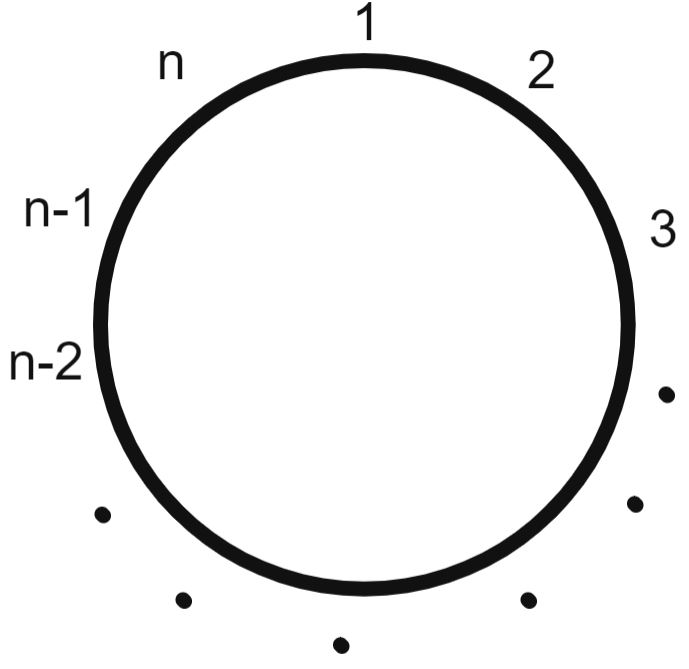
\includegraphics[width=\linewidth]{sol3} %тут поменять имя пикчи
    \end{figure}
    \end{minipage}
\end{minipage}

\textbf{Дефолтные математические знаки и символы:}\\
$\geqslant$,
$\leqslant$,
$a^{b}$,
$x_{i}$,
$\sqrt{a}$,
$\frac{a}{b}$,
$\displaystyle \frac{a}{b}$,
$\cdot$
$\;\Rightarrow\;$,
$\;\Leftrightarrow\;$,
$1{,}2$.
О промежутках:
$a\!b$,
$a\,b$,
$a\:b$,
$a\;b$,
$a\quad b$.

\textbf{Стандартные система и совокупность уравнений / неравенств:}\\
$\left\{
\begin{aligned}
f(x) &= 0 \\
g(x) &= 1
\end{aligned}\right.$

$\left[\begin{aligned}
&\left\{\begin{aligned}
f(x) &\geqslant a \\
g(x) &= b
\end{aligned}\right.\\
&\left\{\begin{aligned}
f(x) &< a \\
g(x) &= -b
\end{aligned}\right.
\end{aligned}\right.$

\subsection*{\textcolor{Emerald}{\textbf{Не математическое, но полезное:}}}
% комментарий в любом месте документа, который нигде не будет видно. Можно использовать для написания заметок-вопросов по задачам
\textbf{Пример таблицы:}

\begin{tabular}{|c|c|c|}
\hline
    $a$ & $b$ & текст
\\\hline
    $c$ & $d$ & мораль
\\\hline
\end{tabular}\\

\textbf{Отступы:} между\smallskip\\ строками\medskip\\ \textbf{Тире} --- это три дефиса.\\
\textbf{Списки:}
\begin{mylist}
\item [$\bullet$] это был пункт а
\item [2)] а это уже пункт номер 2 с изменённым заголовком
\end{mylist}

\subsection*{\textcolor{Emerald}{\textbf{Всё, неупомянутое выше (или если просто что-то не так):}}}
\begin{mylist}
\item [$\bullet$] Решение отдельных вопросов касательно ТеХа нужно искать в \href{https://www.mccme.ru/free-books/llang/newllang.pdf}{Львовском}.

\item [$\bullet$] Найти произвольный символ, который нужен, можно в \href{http://detexify.kirelabs.org/classify.html}{Detexify}.

\item [$\bullet$] Если возникли сомнения при решении, ответ практически ко всем задачам можно проверить с помощью \href{https://www.wolframalpha.com/}{WolframAlpha}.

\item [$\bullet$] Если в задаче нужно создать картинку, то лучше пока отложить эту задачу. Все графики планируется централизованно нарисовать (или перерисовать) в геогебре.

\item [\textcolor{brown}{\textbf{!!}}] Важно ставить \textcolor{red}{\textbf{$\spadesuit$}}
(или просто red) в тело задачи в случае серьёзных вопросов к решению и какой-то вопиющей лажи.

\item [\textcolor{brown}{\textbf{!!}}] Важно ставить \textcolor{olive}{\textbf{$\spadesuit$}}
(или просто olive) в тело задачи в случае не самого удачного текста и кривых отступов.
\end{mylist}

\subsection*{\textcolor{Violet}{\textbf{Комментарии:}}}% а также невидимые комментарии - так можно оставлять заметки-вопросы прямо в задаче, чтобы потом было понятно, в чём вопрос.
\begin{mylist}
\item [$\skull$] Переставлять задачи местами --- очень плохая идея.

\item [$\smiley$] При двойном клике по тексту pdf справа происходит автоматический переход к этому месту в латех-коде, а для обратного перехода можно нажать стрелку вправо (висит сверху между pdf и латех-кодом).

\item [$\smiley$] Если есть размышления, дописывать red/olive к задаче или не дописывать, то лучше всё-таки дописать.

\item [$\skull$] Самое плохое, что можно сделать --- написать в любое поле из трёх (НаписанноеРешение/ВерныйОтвет/Подсказка) только половину того, что надо, никак это не отметить, и потом пойти дальше.\\ Нужно в этот момент писать red/olive в случайном месте задачи, чтобы потом вычислить это с помощью Ctrl+F по всему документу (и это то, что потом будет делаться долго и тщательно)
\end{mylist}

\newpage
\setcounter{num}{963}

\hypertarget{8.6}{{\centering\section*{\bigskip\\\textcolor{Blue}{\hyperlink{start2}{\textcolor{Blue}{8.6}} Алгебраические уравнения.}\vspace{-5mm}}}}

\begin{problem}{Теорема Безу и обратная к ней. Схема Горнера.}{8.6.2}{79I}{(лёгкая)}
{Решить уравнение: $x^{3} - 6x + 5 = 0$.}
{Представим $-6x$, как $-x-5x$:\\
$x^3-6x+5 = x^3-x-5x+5 = 0$.\\
Тогда $x^3-x$ можно представить в виде $x(x^2-1) = x(x-1)(x+1)$, а $-5x+5$, как $-5(x-1)$. Тогда после всех преобразований получим:\\
$x(x-1)(x+1)-5(x-1)=0$.\\
Вынесем $x-1$ за скобки:\\
$(x-1)(x(x+1)-5) = 0$\\
Произведение будет равно 0, если хотя бы один из множителей равен 0:\\
1) $x-1=0 \;\Rightarrow\; x=1$.\\
2) $x(x+1)-5=0 \;\Rightarrow\; x^2+x-5=0$. Решаем квадратное уравнение, получаем:\\
$x = \frac{-1-\sqrt{21}}{2}$, $x = \frac{-1+\sqrt{21}}{2}$.}
{Уравнение $x^3-6x+5=0$ имеет три корня: $x = 1$, $x = \frac{-1+\sqrt{21}}{2}$, $x = \frac{-1-\sqrt{21}}{2}$.}{Представь $-6x$ как $-x-5x$.}
\end{problem}

\begin{problem}{Теорема Безу и обратная к ней. Схема Горнера.}{8.6.2}{9I red разложение на множители}{(лёгкая)}
{Найти произведение и сумму всех действительных корней уравнения $2x^{3} - 2x^{2} - x + 3 = 0$.}
{НаписанноеРешение}
{ВерныйОтвет}{Подсказка}
\end{problem}

\begin{problem}{Метод разложения на множители.}{8.6.3}{79I}{(лёгкая)}
{Решить уравнение с помощью разложения на множители: $x^{3} - 26x^{2} + 25x = 0$.}
{Вынесем $x$ за скобки, получим:\\
$x^3-26x^2+25x = x(x^2-26x+25) = 0$.\\
Тогда:\\
1) $x=0$\\
2) $x^2-26x+25=0 \;\Rightarrow\;$ по теореме Виета сумма корней 26, произведение 25. Легко заметить, что $x = 25$ и $x = 1$.}
{Уравнение имеет 3 корня: $x = 0$, $x = 1$ и $x = 25$.}{Вынеси $x$ за скобки.}
\end{problem}

\begin{problem}{Метод разложения на множители.}{8.6.3}{79I}{(лёгкая)}
{Решить уравнение c помощью разложения на множители: $x^{3} + 3x^{2} + 6x + 8 = 0$.}
{Вынесем $x$ за скобки, получим:\\
$x^3-26x^2+25x = x(x^2-26x+25) = 0$.\\
Тогда:\\
1) $x=0$\\
2) $x^2-26x+25=0 \;\Rightarrow\;$ по теореме Виета сумма корней 26, произведение 25. Легко заметить, что $x = 25$ и $x = 1$.}
{Уравнение имеет 3 корня: $x = 0$, $x = 1$ и $x = 25$.}
{Подсказка}
\end{problem}

\begin{problem}{Метод разложения на множители.}{8.6.3}{79I}{(лёгкая)}
{Решить уравнение c помощью разложения на множители: $x^{3} - 17x = 4x^{2} - 68$.}
{Перенесём всё в левую часть уравнения.\\ Вынесем множитель $x^2$ у cлагаемых при $x^3$ и $4x^2$, и $17$ у $17x$ и $68$: получаем, что \\
$x^3-4x^2-17x+68 = x^2(x-4)-17(x-4)$. Теперь вынесем общий множитель $(x-4)$ за скобки, в итоге получаем: $(x-4)(x^2-17) = 0$.\\ Данное уравнение равно $0$, если а) $x-4 = 0$ или б) $x^2-17 = 0$.\\
а) $x-4 = 0 \;\Rightarrow\; x = 4$.\\
б) $x^2-17 = 0 \;\Rightarrow\; x^2 = 17 \;\Rightarrow\; x = \pm \sqrt{17}$.}
{Уравнение имеет 3 корня: $x = 4$, $x = \sqrt{17},$ и $x = -\sqrt{17}$.}{В этом уравнении можно вынести общие множители у некоторых слагаемых.}
\end{problem}

\begin{problem}{Метод разложения на множители.}{8.6.3}{79I}{(лёгкая)}
{Решить уравнение, разложив на множители: $5x^{3} - 15x^{2} = 9x^{2} - 31x + 12$.}
{1) Разложим на множители левую часть уравнения.\\ Вынесем $5x^2$, получаем: $5x^3-15x^2 = 5x^2(x-3)$.\\
2) Разложим на множители правую часть уравнения. Найдем корни этого многочлена, решив уравнение $9x^2-31x+12 = 0$. Получим два корня: $x = 3$ и $x = \frac{4}{9}$. Тогда этот многочлен представим в виде:\\
$9x^2-31x+12 = 9(x-3)(x-\frac{4}{9}) = (x-3)(9x-4)$.\\
В итоге получаем:\\
$5x^2(x-3) = (x-3)(9x-4)$. Перенесем все в одну часть и вынесем $(x-3)$:\\
$5x^2(x-3)-(x-3)(9x-4) = (x-3)(5x^2-9x+4) = 0$.\\ Данное уравнение равно $0$, если а) $(x-3) = 0$ или б) $5x^2-9x+4 = 0$.\\
а) $x-3 = 0 \;\Rightarrow\; x = 3$.\\
б) $5x^2-9x+4 = 0$. Решаем это уравнение, получаем два корня: $x = 1$ и $x = \frac{4}{5}$.}
{Уравнение имеет 3 решения: $x = 3$, $x = 1$ и $x = \frac{4}{5}$.}{Разложи на множители отдельно левую и правую части.}
\end{problem}

\begin{problem}{Метод разложения на множители.}{8.6.3}{79I}{(лёгкая)}
{Решить уравнение c помощью разложения на множители: $8x^{3} + 27 = 12x^{2} + 18x$.

}
{Для разложения на множители левой части уравнения используем формулу сокращённого умножения: как нам известно, $a^3 + b^3 = (a + b)(a^2 - ab + b^2)$. В нашем случае, $8x^{3} + 27 = (2x + 3)(4x^2 - 6x + 9)$. Разложим на множители и правую часть уравнения: $12x^{2} + 18x = 6x(2x + 3)$.\\ В итоге получаем, что:
$(2x + 3)(4x^2 - 6x + 9) = 6x(2x + 3)$. Следовательно,\\ $(2x + 3)(4x^2 - 6x + 9) - 6x(2x + 3) = 0$. Выносим $(2x+3)$ за скобки:\\
$(2x+3)(4x^2-6x+9-6x) = (2x+3)(4x^2-12x+9) = 0$.\\ Уравнение равно $0$ в том случае, если а) $2x+3 = 0 \;\Rightarrow\; x = -\frac{3}{2}$ или если \\б) $4x^2-12x+9 = 0 \;\Rightarrow\; (2x - 3)^2 = 0 \;\Rightarrow\; x = \frac{3}{2}$.}
{Данное уравнение имеет 2 корня: $x = -\frac{3}{2}$ и $x = \frac{3}{2}$.}{Используй формулу суммы кубов для того, чтобы разложить выражение в левой части уравнения на множители.}
\end{problem}

\begin{problem}{Метод разложения на множители.}{8.6.3}{9I}{(лёгкая)}
{Найти сумму корней уравнения $x^{3} - 8x^{2} + 40 = 0$.}
{Попробуем угадать один корень. Уравнение несложное, поэтому первый корень с легкостью угадывается~--- это $x = -2$. Теперь мы можем разложить это уравнение на множители, поделив его на $(x+2)$. Сделаем это с помощью метода неопределенных коэффициентов:\\
$x^3-8x^2+40 = (Ax^2+Bx+C)(x+2) = Ax^3+Bx^2+Cx+2Ax^2+2Bx+2c \;\Rightarrow\; 
\left(\begin{aligned}
    \: A = 1\\
    \: B+2A = -8 \;\Rightarrow\; B = -10\\
    \: 2C = 40 \;\Rightarrow\; C = 20\\
\end{aligned}\right.$\\
~\\
$x^3-8x^2+40 = (x+2)(x^2-10x+20)$.\\
По теореме Виета сумма корней многочлена $x^2-10x+20$ равна $10$, значит сумма корней изначального уравнения равна $10-2 = 8$.}
{Сумма корней уравнения равна $8$.}{Подсказка}
\end{problem}

\begin{problem}{Метод разложения на множители.}{8.6.3}{9D red многопунктовая}{(лёгкая)}
{Решить уравнение, используя разложение на множители с помощью т. Безу:\\
a) $-x^{3} + 13x^{2} - 30x = 0$\hfill
b) $x^{3} - 4x^{2} - 7x + 10 = 0$\\
c) $x^{3} + 21x^{2} + 71x + 51 = 0$\hfill
d) $x^{4} + x^{3} - 13x^{2} - x + 12 = 0$\\
e) $6x^{4} - 13x^{3} - 8x^{2} + 17x + 6 = 0$ \hfill
f) $24x^{5} - 18x^{4} - 135x^{3} + 39x^{2} + 90x = 0$\\
g) $25x^{5} - 30x^{4} - 101x^{3} + 126x^{2} + 4x - 24 = 0$ \\
h) $x^{9} - 9x^{8} + 30x^{7} - 38x^{6} - 19x^{5} + 99x^{4} - 60x^{3} - 52x^{2} + 48x = 0$}
{a) Несложно заметить, что для коэффициентов верно $1 + 71 = 21 + 51$ (сумма коэффициентов при чётных степенях равна сумме коэффициентов при нечётных степенях)~--- это признак того, что $x = -1$ является корнем.\\ Разделим многочлен $x^{3} + 21x^{2} + 71x + 51$ на $x + 1$:\\
$x^{3} + 21x^{2} + 71x + 51 = (x + 1) \cdot (x^2 + 20x + 51)$.\\ Таким образом, либо $x + 1 = 0$, либо $x^2 + 20x + 51 = 0$.\\ Данное квадратное уравнение можно решить по теореме Виета: $x^2 + 20x + 51 = (x + 3)(x + 17)$. Таким образом, $x^{3} + 21x^{2} + 71x + 51 = (x + 1)(x + 3)(x + 17) = 0$.\medskip\\
b) В данном случае сумма коэффициентов многочлена 4 степени равна 0, поэтому $x = 1$ является корнем, делим на $x - 1$:\\ $x^{4} + x^{3} - 13x^{2} - x + 12 = (x - 1)(x^3 + 2x^2 - 11x - 12)$.\\
Многочлен $x^3 + 2x^2 - 11x - 12$ также легко раскладывается на множители: достаточно заметить, что знакопеременная сумма коэффициентов равна 0 и $x = -1$ является корнем.\\ Раскладываем:
$\;x^3 + 2x^2 - 11x - 12 = (x + 1)(x^2 + x - 12)$.\\ Полученное квадратное уравнение $x^2 + x - 12 = 0$ решим через дискриминант: $D = 1 + 48 = 49 \;\Rightarrow\; x = \frac{-1 \pm 7}{2} = -4; 3$.\\
Итого: $\;x^{4} + x^{3} - 13x^{2} - x + 12 = (x - 1)(x + 1)(x - 3)(x + 4) = 0$.}
{Уравнение $x^{3} + 21x^{2} + 71x + 51 = 0$ имеет три корня: $x = -17$, $x = -3$ и $x = -1$.\medskip\\
Уравнение $x^{4} + x^{3} - 13x^{2} - x + 12 = 0$ имеет 4 корня: $x = -4$, $x = -1$, $x = 1$, и $x = 3$.}{Подсказка}
\end{problem}

\begin{problem}{Метод замены. Биквадратные, симметрические и возвратные уравнения.}{8.6.4}{7A}{(лёгкая)}
{Сколько корней имеет уравнение $(4x^{2} - 6x + 1)^{2} + 8x^{2} - 10(x + 3) - 2x - 3 = 0$?}
{НаписанноеРешение}
{ВерныйОтвет}{Подсказка}
\end{problem}

\begin{problem}{Метод замены. Биквадратные, симметрические и возвратные уравнения.}{8.6.4}{79I}{(лёгкая)}
{Решить квадратное уравнение с модулем: $x^{2} + 3|x| = 28$.}
{Раскроем модуль: сначала для $x \geqslant 0$, не меняя знака выражения, потом для x < 0, со сменой знака:\\
1) $x \geqslant 0$, тогда раскрываем модуль, не меняя знак:\\
$x^2+3x=28 \;\Rightarrow\ x^2+3x-28=0 $\\
Решаем квадратное уравнение, получаем два корня $x = 4$ и $x = -7$, но $x = -7$ нам не подходит, так как мы рассматривали $x \geqslant 0$.\\
2) $x < 0$, тогда раскрываем модуль со сменой знака.\\
$x^2-3x = 28 \;\Rightarrow\ x^2-3x-28 = 0$\\
Решаем квадратное уравнение, получаем $x = -4$, $x = 7$, но $x = 7$ нам не походит, так как мы рассматривали $x < 0$.}
{Уравнение $x^2+|3x|=28$ имеет 2 корня: $x = 4$, $x =-4$}{Раскрой модуль.}
\end{problem}

\begin{problem}{Метод замены. Биквадратные, симметрические и возвратные уравнения.}{8.6.4}{79I}{(лёгкая)}
{Решить уравнение с модулем: $2s^{2} - 5 = -9|s|$.}
{Перенесем модуль в левую часть и раскроем: сначала для $s \geqslant 0$, не меняя знака выражения, потом для s < 0 со сменой знака:\\
$2s^2+9|s|-5 = 0$\\
1) $s \geqslant 0$, тогда:\\
$2s^2+9s-5=0$, решаем квадратное уравнение, получаем $s = -5$, $s = 0.5$, но $s = -5$ не подходит, так как мы рассматривали $s \geqslant 0$.\\
2) $s < 0$, тогда:\\
$2s^2-9s-5 = 0$, решаем квадратное уравнение, получаем $s = 5$, $s = -0.5$, но $x = 5$ нам не подходит, так как мы рассматривали $s < 0$.}
{Уравнение $2s^2-5 = -9|s|$ имеет два корня: $s = 0.5$ и $s = -0.5$.}{Перенеси модуль в левую часть и раскрой его.}
\end{problem}

\begin{problem}{Метод замены. Биквадратные, симметрические и возвратные уравнения.}{8.6.4}{79I}{(лёгкая)}
{Решить уравнение с модулем: $15t^{2} + 8 = 22|t|$.}
{Перенесем модуль в левую часть и раскроем: сначала для $t \geqslant 0$, не меняя знака выражения, потом для t < 0 со сменой знака:\\
$15t^2-22|t|+8 = 0$\\
1) $t \geqslant 0$, тогда:\\
$15t^2-22t+8 = 0$, решаем квадратное уравнение, получаем $t = \frac{2}{3}$, $t = \frac{4}{5}$.\\
2) $t < 0$, тогда:\\
$15t^2+22t+8=0$, решаем квадратное уравнение, получаем $t = -\frac{2}{3}$, $t = -\frac{4}{5}$.}
{Уравнение $15t^2+8 = -22|t|$ имеет 4 корня: $t = \frac{2}{3}$, $t = -\frac{2}{3}$, $t = \frac{4}{5}$, $t = -\frac{4}{5}$}{Перенси модуль в левую часть и раскрой.}
\end{problem}

\begin{problem}{Метод замены. Биквадратные, симметрические и возвратные уравнения.}{8.6.4}{79I}{(лёгкая)}
{Решить уравнение с модулем: $\displaystyle 2x^{2} - 23|x| + 65 = 0$.}
{Раскроем модуль: сначала для $x \geqslant 0$, не меняя знака выражения, потом для x < 0, со сменой знака:\\
$2x^2-23|x|+65 = 0$\\
1) $x \geqslant 0$, тогда:\\
$2x^2-23x+65 = 0$, решаем квадратное уравнение, получаем $x = \frac{13}{2}$, $x = 5$.\\
2) $x < 0$, тогда:\\
$2x^2+23x+65 = 0$, решаем квадратное уравнение, получаем $x = -\frac{13}{2}$, $x = -5$.}
{Уравнение $2x^2-23|x|+65 = 0$ имеет 4 корня: $x = \frac{13}{2}$, $x = -\frac{13}{2}$, $x = 5$, $x = -5$}{Раскрой модуль}
\end{problem}

\begin{problem}{Метод замены. Биквадратные, симметрические и возвратные уравнения.}{8.6.4}{79I}{(лёгкая)}
{Решить уравнение с модулем: $\displaystyle 2x^{2} + |x| - 55 = 0$.}
{Раскроем модуль: сначала для $x \geqslant 0$, не меняя знака выражения, потом для x < 0, со сменой знака:\\
$2x^2+|x|-55 = 0$\\
1) $s \geqslant 0$, тогда:\\
$2x^2+x-55 = 0$, решаем квадратное уравнение, получаем $x = -\frac{11}{2}$, $x = 5$, но $x = -\frac{11}{2}$ не подходит, так как мы рассматривали $x \geqslant 0$.\\
2) $x < 0$, тогда:\\
$2x^2-x-55 = 0$, решаем квадратное уравнение, получаем $x = \frac{11}{2}$, $x = -5$, но $x = \frac{11}{2}$ нам не подходит, так как мы рассматривали $x < 0$.}
{Уравнение $2x^2+|x|-55=0$ имеет два корня: $x = 5$ и $x = -5$.}{Раскрой модуль.}
\end{problem}

\begin{problem}{Метод замены. Биквадратные, симметрические и возвратные уравнения.}{8.6.4}{79I}{(лёгкая)}
{Решить уравнение с модулем: $\displaystyle x^{2} - 2|x| - 63 = 0$.}
{Раскроем модуль: сначала для $x \geqslant 0$, не меняя знака выражения, потом для x < 0, со сменой знака:\\
$x^2-2|x|-63 = 0$\\
1) $s \geqslant 0$, тогда:\\
$x^2-2x-63 = 0$, решаем квадратное уравнение, получаем $x = -7$, $x = 9$, но $x = -7$ не подходит, так как мы рассматривали $x \geqslant 0$.\\
2) $x < 0$, тогда:\\
$x^2+2x-63 = 0$, решаем квадратное уравнение, получаем $x = 7$, $x = -9$, но $x = 7$ нам не подходит, так как мы рассматривали $x < 0$.}
{Уравнение $x^2-2|x|-63 = 0$ имеет два корня: $x = 9$ и $x = -9$.}{Раскрой модуль.}
\end{problem}

\begin{problem}{Метод замены. Биквадратные, симметрические и возвратные уравнения.}{8.6.4}{79I}{(лёгкая)}
{Решить уравнение: $81x^{4} - 16x^{2} = 0$.}
{Вынесем $x^2$, получим:\\
$81x^4-16x^2 = x^2(81x^2-16) = 0$\\
Произведение равно нулю, если хотя бы один из множителей равен нулю:\\
1) $x^2=0 \;\Rightarrow\ x = 0$.\\
2) $81x^2-16 = 0 \;\Rightarrow\ x^2 = \frac{16}{81} \;\Rightarrow\ x = \pm \frac{4}{9}$.}
{Уравнение $81x^4-16x^2 = 0$ имеет 3 корня: $x = 0$, $x = \frac{4}{9}$, $x = -\frac{4}{9}$.}{Вынеси $x^2$.}
\end{problem}

\begin{problem}{Метод замены. Биквадратные, симметрические и возвратные уравнения.}{8.6.4}{79I}{(лёгкая)}
{Решить биквадратное уравнение: $9x^{4} + 8x^{2} - 1 = 0$.}
{Заметим, что если сделать замену $t = x^2$, то уравнение сведется к квадратному:\\
$9x^4+8x^2-1 = 9t^2+8t-1 = 0$, решаем квадратное уравнение относительно $t$, получаем $t = \frac{1}{9}$ и $t = -1$. Делаем обратную замену $x = \sqrt{t}$:\\
1) $t = \frac{1}{9} \;\Rightarrow\ x^2 = \frac{1}{9} \;\Rightarrow\ x = \pm\frac{1}{3}$.\\
2) $t = -1 \;\Rightarrow\ $ вещественных корней нет.}
{Уравнение $9x^4+8x^2-1=0$ имеет 2 вещественных корня: $x = \frac{1}{3}$ и $x = -\frac{1}{3}$. }{Сделай замену $t = x^2$.}
\end{problem}

\begin{problem}{Метод замены. Биквадратные, симметрические и возвратные уравнения.}{8.6.4}{79I}{(лёгкая)}
{Решить уравнение: $2x^{4} - 5x^{2} + 3 = 0$.}
{Заметим, что если сделать замену $t = x^2$, то уравнение сведется к квадратному:\\
$2x^4-5x^2+3 = 2t^2-5t+3 = 0$, решаем квадратное уравнение относительно $t$, получаем $t = \frac{3}{2}$ и $t = 1$. Делаем обратную замену $x = \sqrt{t}$:\\
1) $t = \frac{3}{2} \;\Rightarrow\ x^2 = \frac{3}{2} \;\Rightarrow\ x = \pm\frac{\sqrt{6}}{2}$.\\
2) $t = 1 \;\Rightarrow\ x^2 = 1 \;\Rightarrow\ x = \pm 1$. }
{Уравнение $2x^4-5x^2+3 = 0$ имеет четыре корня: $x = \frac{\sqrt{6}}{2}$, $x = -\frac{\sqrt{6}}{2}$, $x = 1$, $x = -1$.}{Сделай замену $t = x^2$.}
\end{problem}

\begin{problem}{Метод замены. Биквадратные, симметрические и возвратные уравнения.}{8.6.4}{79I}{(лёгкая)}
{Решить уравнение: $(x + 2)^{4} + 5(x + 2)^{2} - 36 = 0$.}
{Очевидно, что выражение $x + 2$ в нашем уравнении повторяется, и логично сделать замену, однако в данном случае оптимально сделать замену $t = (x + 2)^{2}$. Получаем уравнение $t^2 + 5t - 36 = 0$, решаем как квадратное.\\ С помощью теоремы Виета: $4 \cdot (-9) = 36$, $4 - 9 = -5 \;\Rightarrow\; (t - 4)(t + 9) = 0 \;\Rightarrow\;\\ t = -9$; $\,t = 4$. Делаем обратную замену, получаем совокупность уравнений: \\
$\left[\begin{aligned}
t &= -9 \\
t &= 4
\end{aligned}\right.\;\Leftrightarrow\; \left[\begin{aligned}
(x + 2)^2 &= -9 \\
(x + 2)^2 &= 4
\end{aligned}\right.\;\Leftrightarrow\; \left[\begin{aligned}
x &\in \varnothing \\
x &= 0 \\
x &= -4
\end{aligned}\right. \;\Rightarrow$ корней всего два: это 0 и $-4$.}
{Данное уравнение имеет 2 корня: $x = -4$ и $x = 0$.}{Сделай замену.}
\end{problem}

\begin{problem}{Метод замены. Биквадратные, симметрические и возвратные уравнения.}{8.6.4}{79I}{*}
{Решить уравнение: $x^{2} + 2x - 40|x + 1| + 112 = 0$.}
{Это уравнение логично решать методом замены: здесь $z = |x + 1|$ (так как $|a|^2 = a^2$). Получаем $z^2 - 40z + 111 = 0 \Leftrightarrow (z - 3)(z - 37) = 0\;$ (теорема Виета + факт, что $111 = 3\cdot37$ из теории делимости). Значит, $z = 3$ или $z = 37$. Получаем совокупность уравнений с модулем:\\
$\left[\begin{aligned}
z &= 3 \\
z &= 37
\end{aligned}\right.\;\Longleftrightarrow\; \left[\begin{aligned}
|x + 1| &= 3 \\
|x + 1| &= 37
\end{aligned}\right.\;\Longleftrightarrow\; \left[\begin{aligned}
x + 1 &= 3 \\
x + 1 &= -3 \\
x + 1 &= 37 \\
x + 1 &= -37
\end{aligned}\right.\;\Longleftrightarrow\; \left[\begin{aligned}
x &= 2 \\
x &= -4 \\
x &= 36 \\
x &= -38
\end{aligned}\right.$}
{Уравнение имеет 4 корня: $x = -38$, $x = -4$, $x = 2$, $x = 36$.}{Сделай замену, чтобы избавиться от модуля.}
\end{problem}

\begin{problem}{Метод замены. Биквадратные, симметрические и возвратные уравнения.}{8.6.4}{79I}{(лёгкая)}
{Решить уравнение: $x^{5} - 5x^{3} - 36x = 0$.}
{НаписанноеРешение}
{ВерныйОтвет}{Подсказка}
\end{problem}

\begin{problem}{Метод замены. Биквадратные, симметрические и возвратные уравнения.}{8.6.4}{8M}{(лёгкая)}
{Решить уравнение $x^{6} - 2x^{4} + x^{2} = 0$.}
{НаписанноеРешение}
{ВерныйОтвет}{Подсказка}
\end{problem}

\begin{problem}{Метод замены. Биквадратные, симметрические и возвратные уравнения.}{8.6.4}{9D}{(лёгкая)}
{Решить возвратное уравнение: $2x^{3} + 7x^{2} + 7x + 2 = 0$.}
{НаписанноеРешение}
{ВерныйОтвет}{Подсказка}
\end{problem}

\begin{problem}{Метод замены. Биквадратные, симметрические и возвратные уравнения.}{8.6.4}{9D}{(лёгкая)}
{Решить уравнение: $6a^{3} - 7a^{2} - 7a + 6 = 0$.}
{НаписанноеРешение}
{ВерныйОтвет}{Подсказка}
\end{problem}

\begin{problem}{Метод замены. Биквадратные, симметрические и возвратные уравнения.}{8.6.4}{9D}{(лёгкая)}
{Решить возвратное уравнение: $6x^3 - 43x^2 + 43x - 6 = 0$.}
{Для решения возвратного уравнения третьей степени сгруппируем \\коэффициенты и применим ФСУ:\\
$6x^3 - 43x^2 + 43x - 6 = 0 \Leftrightarrow 6(x^3 - 1) - 43x(x - 1) = 0 \Leftrightarrow 6(x - 1)(x^2 + x + 1) - 43x(x - 1) = 0 \Leftrightarrow (x - 1)(6x^2 + 6x + 6 - 43x) = 0 \Leftrightarrow (x - 1)(6x^2 - 37x + 6) = 0$.\smallskip\\
Мы нашли корень $x = 1$, теперь ищем корни у квадратного уравнения $6x^2 - 37x + 6 = 0$. $\;D = 37^2 - 4\cdot36 = (37 + 2\cdot6)\cdot(37 - 2\cdot6) = 49\cdot25$. Корень извлекается.\\ $x = \frac{37 \pm 7\cdot5}{12} = 6; \frac16$.}
{Уравнение имеет 3 корня: $x = \frac16$, $x = 1$, $x = 6$.}{Сгруппируй коэффициенты и разложи выражение на множители.}
\end{problem}

\begin{problem}{Метод замены. Биквадратные, симметрические и возвратные уравнения.}{8.6.4}{9D}{(лёгкая)}
{Решить возвратное уравнение: $6x^{4} - 25x^{3} + 12x^{2} + 25x + 6 = 0$.}
{Для решения возвратного уравнения 4 степени предварительно поделим на $x^2$: так как свободный член равен 6, $x = 0$ не является корнем.\\ $6x^{4} - 25x^{3} + 12x^{2} + 25x + 6 = 0 \;\Rightarrow\; 6x^2 - 25x + 12 + \frac{25}{x} + \frac{6}{x^2} = 0 \;\Leftrightarrow\; 6\cdot\left(x^2 + 2 + \frac{1}{x^2}\right) - 25\left(x - \frac{1}{x}\right) = 0 \;\Leftrightarrow\; 6\cdot\left(x - \frac{1}{x}\right)^2 - 25\left(x - \frac{1}{x}\right) + 24 = 0$.\smallskip\\
Делаем замену $y = x - \frac{1}{x}$. Получаем уравнение $y^2 - 25y + 24 = (y - 1)(y - 24) = 0$.\\
Следовательно, $\left[\begin{aligned}
y &= 1 \\
y &= 24
\end{aligned}\right.\;\Longleftrightarrow\; \left[\begin{aligned}
x - \frac{1}{x} &= 1 \\
x - \frac{1}{x} &= 24
\end{aligned}\right.\;\Longleftrightarrow\; \left[\begin{aligned}
x^2 - 1 &= x \\
x^2 - 1 &= 24x
\end{aligned}\right.\;\Longleftrightarrow\;\\ \left[\begin{aligned}
x^2 - x - 1 &= 0 \\
x^2 - 24x - 1 &= 0 
\end{aligned}\right.\;\Longleftrightarrow\; \left[\begin{aligned}
x &= \frac{1 \pm \sqrt{5}}{2} \\
x &= \frac{24 \pm \sqrt{580}}{2}
\end{aligned}\right.\;\Longleftrightarrow\; \left[\begin{aligned}
x &= \frac{1 \pm \sqrt{5}}{2} \\
x &= 12 \pm \sqrt{145}
\end{aligned}\right.$}
{Уравнение имеет 4 корня: $\displaystyle x = \frac{1 - \sqrt{5}}{2}$, $x = 12 - \sqrt{145}$, $\displaystyle x = \frac{1 + \sqrt{5}}{2}$, $x = 12 + \sqrt{145}$.}{Деление на $x^2$, группировка, замена.}
\end{problem}

\begin{problem}{Метод замены. Биквадратные, симметрические и возвратные уравнения.}{8.6.4}{9D}{(лёгкая)}
{Решить возвратное уравнение: $x^{4} + 13x^{3} + 38x^{2} + 13x + 1 = 0$.}
{Для того чтобы решить возвратное уравнение четвёртой степени поделим на $x^2$: так как свободный член равен 1, $x = 0$ не является корнем. Получаем:\smallskip\\ $x^{4} + 13x^{3} + 38x^{2} + 13x + 1 = 0 \;\Rightarrow\; x^2 + 13x + 38 + \frac{13}{x} + \frac{1}{x^2} = 0 \;\Leftrightarrow\;\\ \left(x + \frac{1}{x}\right)^2 + 13\left(x + \frac{1}{x}\right) + 36 = 0.$\smallskip\\
Делаем замену $y = x + \frac{1}{x}$. Получаем уравнение $y^2 + 13y + 36 = (y + 4)(y + 9) = 0$.\\
Следовательно, $\left[\begin{aligned}
y &= -9 \\
y &= -4
\end{aligned}\right.\;\Longleftrightarrow\; \left[\begin{aligned}
x + \frac{1}{x} &= -9 \\
x + \frac{1}{x} &= -4
\end{aligned}\right.\;\Longleftrightarrow\; \left[\begin{aligned}
x^2 + 1 &= -9x \\
x^2 + 1 &= -4x
\end{aligned}\right.\;\Longleftrightarrow\;$\smallskip\\
$\left[\begin{aligned}
x^2 + 9x + 1 &= 0 \\
x^2 + 4x + 1 &= 0 
\end{aligned}\right.\;\Longleftrightarrow\; \left[\begin{aligned}
x &= \frac{-9 \pm \sqrt{77}}{2} \\
x &= \frac{-4 \pm \sqrt{12}}{2}
\end{aligned}\right.\;\Longleftrightarrow\; \left[\begin{aligned}
x &= \frac{-9 \pm \sqrt{77}}{2} \\
x &= -2 \pm \sqrt{3}.
\end{aligned}\right.$}
{Уравнение имеет 4 корня: $\displaystyle x = \frac{-9 \pm \sqrt{77}}{2}$, $\;\displaystyle x = -2 \pm \sqrt{3}$.}{Деление на $x^2$, группировка, замена.}
\end{problem}

\begin{problem}{Метод замены. Биквадратные, симметрические и возвратные уравнения.}{8.6.4}{9D}{(лёгкая)}
{Решить уравнение: $\displaystyle (x^{2} - 8x + 11)^{2} - 24x^{2} + 192x - 184 = 0$.}
{При раскрытии скобок мы получим уравнение 4-ой степени, которое мы не умеем решать. Поэтому вместо этого попробуем сгруппировать слагаемые и сделать замену $y = x^2 - 8x + 11$ (хотя и $z = x^2 - 8x$ тоже вариант не хуже).\smallskip\\
$(x^{2} - 8x + 11)^{2} - 24x^{2} + 192x - 184 = (x^{2} - 8x + 11)^{2} - 24(x^2 - 8x + 11) + 264 - 184 = $\\
$y^2 - 24y + 80 = 0 \;\Rightarrow\; (y - 20)(y - 4) = 0 \;\Rightarrow\; \left[\begin{aligned}
y &= 4\\
y &= 20
\end{aligned}\right. \;\Rightarrow\; \left[\begin{aligned}
x^{2} - 8x + 11 &= 4\\
x^{2} - 8x + 11 &= 20
\end{aligned}\right. \;\Rightarrow$ \\
$\left[\begin{aligned}
x^{2} - 8x + 7 &= 0\\
x^{2} - 8x - 9 &= 0
\end{aligned}\right. \;\Rightarrow\; \left[\begin{aligned}
(x - 1)(x - 7) &= 0\\
(x - 9)(x + 1) &= 0
\end{aligned}\right. \;\Rightarrow\; x = -1;\; x = 1;\; x = 7;\; x = 9$.}
{Уравнение имеет 4 корня: $x = -1;\; x = 1;\; x = 7;\; x = 9$.}{Здесь можно (и нужно) сделать замену.}
\end{problem}

\begin{problem}{Метод замены. Биквадратные, симметрические и возвратные уравнения.}{8.6.4}{9D}{(лёгкая)}
{Решить уравнение: $\displaystyle (x^{2} + 14)^{2} - 3x^{2} - 46 = 0$.}
{НаписанноеРешение}
{ВерныйОтвет}{Подсказка}
\end{problem}

\begin{problem}{Метод замены. Биквадратные, симметрические и возвратные уравнения.}{8.6.4}{9D}{(лёгкая)}
{Решить уравнение: $\displaystyle (x^{2} - 2x - 1)^{2} + 3x^{2} - 6x - 13 = 0$.}
{Выделим полный квадрат в $x^2-2x-1 = (x-1)^2-2$ и $3x^2-6x-13 = 3((x-1)^2-\frac{16}{3}) = 3(x-1)^2-16$. Тогда будет удобно сделать замену $(x-1)^2 = t$. Получим:\\
$((x-1)^2-2)^2+3(x-1)^2-16 = t^2-4t-4+3t+16 = t^2-t+12$. Решаем квадратное уравнение относительно $t$, получаем два корня: $t = 4$ и $t = -3$.\\
1) $t = 4 \;\Rightarrow\; (x-1)^2 = 4 \;\Rightarrow\; x = 3$ и $x = -1$.\\
2) $t = -2 \;\Rightarrow\;$ вещественных решений для $x$ нет.}
{Уравнение имеет два вещественных решения: $x = 3$ и $x = -1$.}{Выдели полные квадраты.}
\end{problem}

\begin{problem}{Метод замены. Биквадратные, симметрические и возвратные уравнения.}{8.6.4}{9D}{(лёгкая)}
{Решить уравнение: $(4 + (x + 2)(3x - 4))^{2} - 15x^{2} - 10x + 24 = 0$.}
{НаписанноеРешение}
{ВерныйОтвет}{Подсказка}
\end{problem}

\begin{problem}{Метод замены. Биквадратные, симметрические и возвратные уравнения.}{8.6.4}{9D}{(лёгкая)}
{Решить уравнение $(x^{2} + x - 33)^{2} + 4(x^{2} + x - 22) - 161 = 0$.}
{Поскольку в нашем уравнении повторяется выражение $x^2 + x$, а других вхождений $x$ нет, логично сделать замену $y = x^2 + x$. Получаем следующее:\\ $(y - 33)^{2} + 4(y - 22) - 161 = 0$. Раскроем скобки: $(y - 33)^{2} + 4(y - 22) - 161 = y^2 - 66y + 1089 + 4y - 88 - 161 = y^2 - 62y + 840 = 0$.\\
Если сработает <<метод соколиного глаза>> и мы по теореме Виета увидим $42 + 20 = 62$ и $42\cdot20 = 840$, то можно сразу перейти к решению совокупности.\\ Если же нет, решаем через дискриминант:\\
$D = 62^2 - 4\cdot840 = 4\cdot(31^2 - 840) = 4\cdot121 \Rightarrow y = \frac{62 \pm 2\cdot11}{2} = 20; 42$.\\
Таким образом, мы получили совокупность уравнений:
$\left[\begin{aligned}
y &= 20 \\
y &= 42
\end{aligned}\right.\Longleftrightarrow \left[\begin{aligned}
x^2 + x &= 20 \\
x^2 + x &= 42
\end{aligned}\right.\\ \left[\begin{aligned}
x^2 + x - 20 &= 0 \\
x^2 + x - 42 &= 0
\end{aligned}\right.\;\Longleftrightarrow\; \left[\begin{aligned}
(x - 4)(x + 5) &= 0 \\
(x - 6)(x + 7) &= 0
\end{aligned}\right.\;\Longleftrightarrow\;
x = -7$; $\;x = -5$; $\;x = 4$; $\;x = 6$.}
{Уравнение $(x^{2} + x - 33)^{2} + 4(x^{2} + x - 22) - 161 = 0$ имеет 4 корня:\\ $x = -7$; $\;x = -5$; $\;x = 4$; $\;x = 6$.}{Сделай замену.}
\end{problem}

\begin{problem}{Метод замены. Биквадратные, симметрические и возвратные уравнения.}{8.6.4}{9D}{*}
{Решить уравнение: $x^{4} + 12x^{3} + 49x^{2} + 78x + 40 = 0$.}
{НаписанноеРешение}
{ВерныйОтвет}{Подсказка}
\end{problem}

\begin{problem}{Метод замены. Биквадратные, симметрические и возвратные уравнения.}{8.6.4}{9D}{(лёгкая)}
{Решить уравнение, выполнив подходящую замену переменной: $$\displaystyle (2x^{2} + 3x - 1)^{2} - 10x^{2} - 15x + 9 = 0.$$

}
{НаписанноеРешение}
{ВерныйОтвет}{Подсказка}
\end{problem}

\begin{problem}{Метод замены. Биквадратные, симметрические и возвратные уравнения.}{8.6.4}{9D}{*}
{Решить уравнение, выполнив подходящую замену переменной: $$\displaystyle \frac{x^{2} - 3x - 6}{x} - \frac{8x}{x^{2} - 3x - 6} = -2.$$

}
{Выполним замену $\frac{x^2-3x-6}{x} = t$, тогда $\frac{8x}{x^2-3x-6} = \frac{8}{t}$. Получим следующее уравнение:\\
$t-\frac{8}{t} = -2$. Перенесем $-2$ налево и домножим на $t$:\\
$t^2+2t-8 = 0$. Корни этого уравнения: $t = 2$ и $t = -4$. Выполним обратную замену:\\
1) $\frac{x^2-3x-6}{x} = 2 \;\Rightarrow\; x^2-5x-6 = 0$. Решаем уравнение, получаем: $x = 6$ и $x = -1$.\\
2) $\frac{x^2-3x-6}{x} = -4 \;\Rightarrow\; x^2+x-6 = 0$. Решаем уравнение, получаем $x = 2$ и $x = -3$.}
{Уравнение имеет 4 решения: $x = -4$, $x = -3$, $x = -1$ и $x = 2$.}{Сделай замену $\frac{x^2-3x-6}{x} = t$. }
\end{problem}

\begin{problem}{Метод замены. Биквадратные, симметрические и возвратные уравнения.}{8.6.4}{9D}{*}
{Решить уравнение: $(x + 1)(x + 2)(x + 4)(x + 5) = 40$.}
{Математические задачи хорошо решаются, если везде появляется одно и то же выражение. В данном случае надо применить следующую хитрость:\\
$(x + 1)(x + 2)(x + 4)(x + 5) = 40 \Longleftrightarrow\; (x + 2)(x + 4) \cdot (x + 5)(x + 1) = 40 \Longleftrightarrow\;$\\
$(x^2 + 6x + 8) \cdot (x^2 + 6x + 5) = 40$.\\
Теперь после замены $z = x^2 + 6x$ и раскрытия скобок мы придём к квадратному уравнению:
$(z + 8)(z + 5) = 40 \Rightarrow z^2 + 13z + 40 = 40 \Rightarrow z(z + 13) = 0 \Rightarrow$ $z = -13$; $z = 0$.\\
Решаем совокупность уравнений:
$\left[\begin{aligned}
z &= -13 \\
z &= 0
\end{aligned}\right.\;\Longleftrightarrow\; \left[\begin{aligned}
x^2 + 6x &= -13 \\
x^2 + 6x &= 0
\end{aligned}\right.\;\Longleftrightarrow\;\\ \left[\begin{aligned}
x^2 + 6x + 13 &= 0 \\
x(x + 6) &= 0
\end{aligned}\right.\;\Longleftrightarrow\; \left[\begin{aligned}
x &\in \varnothing \\
x(x + 6) &= 0
\end{aligned}\right.\;\Longleftrightarrow\;
x = -6$; $\;x = 0$.}
{Уравнение $(x + 1)(x + 2)(x + 4)(x + 5) = 40$ имеет 2 корня: \\$\;x = -6\,$ и $\,x = 0$.}{В данной задаче стоит использовать симметрию и раскрыть скобки в другом порядке, а уже потом сделать замену.}
\end{problem}

\begin{problem}{Метод замены. Биквадратные, симметрические и возвратные уравнения.}{8.6.4}{9D}{*}
{Решить уравнение: $(x + 1)(x + 3)(x + 5)(x + 7) = 48$.}
{НаписанноеРешение}
{ВерныйОтвет}{Подсказка}
\end{problem}

\begin{problem}{Метод замены. Биквадратные, симметрические и возвратные уравнения.}{8.6.4}{9D}{*}
{Решить уравнение: $(x + 1)(x + 2)(x + 3)(x + 4) = 100$.}
{НаписанноеРешение}
{ВерныйОтвет}{Подсказка}
\end{problem}

\begin{problem}{Рациональные уравнения.}{8.6.5}{X}{(лёгкая)}
{Решить уравнение: $\;\displaystyle x = \frac{8x - 35}{x - 4}$.}
{$x = 4$ не является решением уравнения: слева получается 4, а выражение справа не определено. Поэтому домножаем обе части уравнения на $x - 4$: получаем, что $x(x - 4) = 8x - 35$, откуда $x^2 - 4x = 8x - 35$. Переносим все слагаемые влево, приводим подобные члены: $\;\Rightarrow\; x^2 - 12x + 35 = 0 \;\Rightarrow\; (x - 5)(x - 7) = 0$ (угадали корни по теореме Виета).\\
Таким образом, данное уравнение имеет два корня: $x = 5$ и $x = 7$.}
{Решениями являются $x = 5$ и $x = 7$.}{Перенеси всё в одну часть уравнения и приведи всё к общему знаменателю (или обоснуй, почему от него можно избавиться).}
\end{problem}

\begin{problem}{Рациональные уравнения.}{8.6.5}{X}{(лёгкая)}
{Решить уравнение на $\gamma$: $\;\displaystyle (\gamma - 2) - \frac{2017}{\gamma - 2} + 1 = 2017$.}
{НаписанноеРешение}
{ВерныйОтвет}{Подсказка}
\end{problem}

\begin{problem}{Рациональные уравнения.}{8.6.5}{X}{(лёгкая)}
{Решить уравнение: $\displaystyle \;\frac{x - 1}{x + 1} = x$.}
{$x = -1$ не является решением уравнения: справа $-1$, а выражение слева не определено. Поэтому домножаем обе части уравнения на $x + 1$: получаем, что $x - 1 = x(x + 1) \;\Rightarrow\; x - 1 = x^2 + x \;\Rightarrow\; x^2 + 1 = 0$. Но для любого $x$ левая часть уравнения будет больше или равна 1, так как $x^2 \geqslant 0$.\\
Значит, решений у даннного уравнения нет ($D = 0^2 - 4\cdot1\cdot1 = -4 < 0$).}
{Данное уравнение не имеет решений.}{Приведи всё к общему знаменателю, собрав всё в одной из частей уравнения. Имеет ли корни полученное квадратное?}
\end{problem}

\begin{problem}{Рациональные уравнения.}{8.6.5}{X}{(лёгкая)}
{Решить уравнение: $\displaystyle\; \frac{1}{x^{2} - 8x - 9} = \frac{1}{3x^{2} + 5x + 2}$.}
{Выясним, когда знаменатели дробей равны 0: тогда дроби не определены и уравнение не имеет смысла: $\left[\begin{aligned}
x^{2} - 8x - 9 &= 0\\
3x^{2} + 5x + 2 &= 0
\end{aligned}\right. \;\Rightarrow\; \left[\begin{aligned}
(x - 9)(x + 1) &= 0\\
(3x + 2)(x + 1) &= 0
\end{aligned}\right.$
$\Rightarrow x \neq -1;\; x \neq -\frac23;\; x \neq 9$.\smallskip\\ Дроби равны тогда, когда равны их ненулевые знаменатели: $ x^{2} - 8x - 9 = 3x^{2} + 5x + 2 \;\Rightarrow\; 2x^2 + 13x + 11 = 0 \;\Rightarrow\; (x + 1)(2x + 11) = 0 \;\Rightarrow\; x = -1; \; x = -5{,}5$.\\ Учитывая, что $x \neq -1$, остаётся только один корень $x = -5{,}5$.}
{Уравнение имеет один корень, $x = -5{,}5$.}{Не забудь отбросить решения, при которых значение какой-то из дробей не определено.}
\end{problem}

\begin{problem}{Уравнения с модулем.}{8.6.6}{9I}{(лёгкая)}
{Решить уравнение $|x - 1| + |x + 2| = 3$.}
{Очевидно, что первый модуль меняет знак первого выражения когда $x < 1$, а второй модуль меняет знак второго выражения когда $x < -2$. \\Поэтому есть всего три случая:\smallskip\\
Случай №1: $x < -2$. Тогда оба модуля раскрываются с другим знаком, и $|x - 1| + |x + 2| = 3 \;\Rightarrow\; 1 - x - x - 2 = 3 \;\Rightarrow\; -2x = 4 \;\Rightarrow\; x = -2$.\\ Но мы рассматривали только $x < -2$, корней нет.\smallskip\\
Случай №2: $-2 \leqslant x < 1$. Тогда первый модуль знак меняет ($x < 1$, выражение под первым модулем отрицательно), а второй модуль знак не меняет ($x \geqslant -2$, выражение под вторым модулем неотрицательно). Раскрывая модули, получаем $1 - x + x + 2 = 3 \;\Rightarrow\; 3 = 3$. То есть мы пришли к тождеству~--- тождественно верному выражению. Любой $x$ является его корнем, так как уравнение остаётся верным. Следовательно, любой $x \in [-2; 1)$ является решением.\smallskip\\
Случай №3: $x \geqslant 1$. Тогда оба модуля раскрываются без изменения знака: $x - 1 + x + 2 = 3 \;\Rightarrow\; 2x = 2 \;\Rightarrow\; x = 1$, этот корень нам подходит.\smallskip\\
Мы рассмотрели все $x \in \mathbb{R}$, и таким образом множество $x$, являющееся решением уравнения~--- это целый отрезок $[-2; 1]$.}
{Решением уравнения является любое число из отрезка $[-2; 1]$.}{Для всех возможных $x \in\mathbb{R}$ нужно рассмотреть три области, в каждой из которых модули раскрываются определённым способом, и в каждой из этих областей найти все подходящие решения.}
\end{problem}

\begin{problem}{Уравнения с модулем.}{8.6.6}{9D}{(лёгкая)}
{Нарисовать график функции $y = |2x - 3| + |x - 4|$.}
{НаписанноеРешение}
{ВерныйОтвет}{Подсказка}
\end{problem}

\begin{problem}{Уравнения с модулем.}{8.6.6}{9D red номер на замену}{(лёгкая)}
{Решить уравнение: $x^{2} + 6x + 7 = |2x + 6| - 2$.}
{Заметим, что $x^{2} + 6x + 7 = |2x + 6| - 2 \;\Longleftrightarrow\; (x + 3)^2 - 2 = 2|x + 3| - 2$.\\
Делаем замену $t = |x + 3|$: $\;t^2 - 2 = 2t - 2 \;\Longleftrightarrow\; t^2 - 2t = 0 \Rightarrow t(t - 2) = 0$.\\
Мы получили совокупность уравнений. Решаем её:\\
$\left[\begin{aligned}
t &= 0 \\
t &= 2
\end{aligned}\right.\;\Longleftrightarrow\; \left[\begin{aligned}
|x + 3| &= 0 \\
|x + 3| &= 2
\end{aligned}\right.\;\Longleftrightarrow\; \left[\begin{aligned}
x + 3 &= 0 \\
x + 3 &= 2 \\
x + 3 &= -2
\end{aligned}\right.\;\Longleftrightarrow\; \left[\begin{aligned}
x &= -3 \\
x &= -1 \\
x &= -5
\end{aligned}\right.\;\Longleftrightarrow\;
x = -5$; $\;x = -3$; $\;x = -1$.}
{Уравнение $x^{2} + 6x + 7 = |2x + 6| - 2$ имеет 3 корня: $\:x = -5$, $\;x = -3\,$ и $\;x = -1$.}{Сделай замену, чтобы избавиться от модуля.}
\end{problem}

\begin{problem}{Уравнения с модулем.}{8.6.6}{9D}{(лёгкая)}
{Решить уравнение: $\;\displaystyle |x - 2| + |x + 3| = 6$.}
{НаписанноеРешение}
{ВерныйОтвет}{Подсказка}
\end{problem}

\begin{problem}{Уравнения с модулем.}{8.6.6}{9D red многопунктовая}{(лёгкая)}
{Определить количество решений уравнения
\\a) $\displaystyle \left|x + \frac{1}{x}\right| = 2$.
\smallskip\\b) $\displaystyle \left|2x + \frac{1}{x}\right| = 3$.}
{НаписанноеРешение}
{ВерныйОтвет}{Подсказка}
\end{problem}

\begin{problem}{Уравнения с модулем.}{8.6.6}{9D}{(лёгкая)}
{Решить уравнение: $\;4 - ||x - 5| - 2| = ||x - 3| - 2|$.}
{НаписанноеРешение}
{ВерныйОтвет}{Подсказка}
\end{problem}

\begin{problem}{Уравнения с модулем.}{8.6.6}{9D}{*}
{Решить уравнение: $|x^{2} - 5| = x + 1$.}
{Рассмотрим, как надо раскрывать модуль в зависимости от $x$: для этого решим неравенство $x^2 - 5 \geqslant 0$: $\;x^2 - 5 \geqslant 0 \Rightarrow x^2 \geqslant 5 \Rightarrow x \in (-\infty; -\sqrt{5}] \cup [\sqrt{5}; +\infty)$. В этой области модуль раскрывается с тем же знаком, а в её дополнении, $x \in (-\sqrt{5}; \sqrt{5})$, знак меняется на противоположный. Следовательно, $|x^{2} - 5| = x + 1 \;\Longleftrightarrow\; \left[\begin{aligned}
&\left\{\begin{aligned}
&x \in (-\infty; -\sqrt{5}] \cup [\sqrt{5}; +\infty) \\
&x^{2} - 5 = x + 1
\end{aligned}\right.\\
&\left\{\begin{aligned}
x \in (-\sqrt{5}; \sqrt{5}) \\
5 - x^{2} = x + 1
\end{aligned}\right.
\end{aligned}\right.\;\Longleftrightarrow\;$\\
$\left[\begin{aligned}
&\left\{\begin{aligned}
&x \in (-\infty; -\sqrt{5}] \cup [\sqrt{5}; +\infty) \\
&x^{2} - x - 6 = 0
\end{aligned}\right.\\
&\left\{\begin{aligned}
x \in (-\sqrt{5}; \sqrt{5}) \\
x^{2} + x - 4 = 0
\end{aligned}\right.
\end{aligned}\right.\;\Longleftrightarrow\;\left[\begin{aligned}
&\left\{\begin{aligned}
&x \in (-\infty; -\sqrt{5}] \cup [\sqrt{5}; +\infty) \\
&(x - 3)(x + 2) = 0
\end{aligned}\right.\\
&\left\{\begin{aligned}
x \in (-\sqrt{5}; \sqrt{5}) \\
x = \frac{-1 \pm \sqrt{17}}{2}
\end{aligned}\right.
\end{aligned}\right.\;\Longleftrightarrow\;\\\left[\begin{aligned}
x &= 3\\
x &= \frac{-1 + \sqrt{17}}{2}
\end{aligned}\right.\;$ (поскольку $-2 > -\sqrt{5}\;$ и $\;\frac{-1 - \sqrt{17}}{2} < \frac{-1 - \sqrt{16}}{2} = -\frac52 < -\sqrt{5}$)}
{Данное уравнение имеет два корня: $x = \frac{-1 + \sqrt{17}}{2}\;$ и $\;x = 3$.}{Рассмотреть оба случая раскрытия модуля, и в каждой области\\ найти подходящее решение.}
\end{problem}

\begin{problem}{Уравнения с модулем.}{8.6.6}{9D}{(лёгкая)}
{Решить уравнение: $\;\displaystyle ||2x - 3| - 1| = x$.}
{НаписанноеРешение}
{ВерныйОтвет}{Подсказка}
\end{problem}

\begin{problem}{Уравнения с модулем.}{8.6.6}{9D}{(лёгкая)}
{Решить уравнение: $\;||4x - 3| - 5| = 2x + 3{,}5$.}
{НаписанноеРешение}
{ВерныйОтвет}{Подсказка}
\end{problem}

\begin{problem}{Уравнения с модулем.}{8.6.6}{9D}{(лёгкая)}
{Решить уравнение: $\;|4x - 7| + |3x - 2| = 6 - x$.}
{НаписанноеРешение}
{ВерныйОтвет}{Подсказка}
\end{problem}

\begin{problem}{Уравнения с модулем.}{8.6.6}{9D}{(лёгкая)}
{Решить уравнение: $\;|1 - x^{2}| = |2x - 2|$.}
{НаписанноеРешение}
{ВерныйОтвет}{Подсказка}
\end{problem}

\begin{problem}{Уравнения с модулем.}{8.6.6}{9D}{(лёгкая)}
{Решить уравнение: $\;||3x - 3| - 2| = 2x$.}
{Сразу заметим, что в левой части модуль, поэтому правая часть должна быть неотрицательной: $x \geqslant 0$. Из внутреннего модуля, для удобства, вынесем множитель $3$: $| 3\cdot|x - 1| - 2| = 2x$. Раскроем модуль $|x - 1|$ сначала для $x$ из интервала $\lbrack0;1)$, а потом для $x$ из интервала $[1;+\infty)$.\\
1) $x \in \lbrack0;1)$, тогда модуль раскрываем со знаком <<$-$>>: $|3 - 3x - 2| = |1 - 3x| = 2x$.\\
Теперь раскроем модуль $|1 - 3x| $ сначала для $x \in (\frac{1}{3};1)$, а потом для $x \in [0;\frac{1}{3})$.\\
а) $x \in (\frac{1}{3};1)$, тогда раскроем модуль со знаком <<$-$>>:\\
$|1 - 3x| = 3x - 1 = 2x \;\Rightarrow\; x = 1$. В наш интервал не попадает, так как концы не включены.\\
б) $x \in [0;\frac{1}{3})$, тогда раскроем модуль со знаком <<$-$>>:\\
$|1 - 3x| = 1 - 3x = 2x \;\Rightarrow\; x = \frac{1}{5}$.\smallskip\\
2) $x \in [1;+\infty)$, тогда модуль раскроем со знаком <<$+$>>:\\
$|3x - 3 - 2| = |3x - 5| = 2x$. Теперь раскроем модуль $3x - 5$ сначала для $x \in [1;\frac{5}{3})$, а потом для $x \in [\frac{5}{3}; +\infty)$.\\
а) $x \in [1;\frac{5}{3})$, тогда раскроем модуль со знаком  <<$-$>>:\\
$|3x - 5| = 5 - 3x = 2x \;\Rightarrow\; x = 1$.\\
б)  $x \in [\frac53; +\infty)$, тогда раскроем модуль со знаком <<$+$>>:\\
$|3x - 5| = 3x - 5 = 2x \;\Rightarrow\; x = 5.$\\
Таким образом, нашлось несколько решений: $x = \frac15$, $x = 1$, $x = 5$.}
{Уравнение имеет три решения: $x = \frac15$, $x = 1$, $x = 5$.}{Раскрой модуль в каждом случае или реши уравнение графически.}
\end{problem}

\begin{problem}{Иррациональные уравнения.}{8.6.7}{79I}{(лёгкая)}
{Решить иррациональное уравнение: $\:\sqrt{12 + x} = x$.}
{Подкоренное выражение неотрицательно, т.е. $12+x \geqslant 0  \;\Rightarrow\; x \geqslant -12$, но в то же время правая часть должна быть неотрицательна, т.е. $x \geqslant 0$ поэтому область допустимых значений этого уравенения $[0;+\infty)$.\\
Возведем в квадрат обе части уравнения. Получим:
$12+x=x^2$. Перенесем все в одну часть и решим квадратное уравнение. Получим два корня: $x = 4$ и $x = -3$. Корень $x = 4$ нам подходит, а корень $x = -3$ не подходит, так как не удовлетворяет ОДЗ.}
{Уравнение имеет один корень: $x = 4$.}{Возведи в квадрат обе части и не забудь про ОДЗ.}
\end{problem}

\begin{problem}{Иррациональные уравнения.}{8.6.7}{79I}{(лёгкая)}
{Решить уравнение: $\:\sqrt{14 - 5x} = x$.}
{Подкоренное выражение неотрицательно, т.е. $14-5x \geqslant 0  \;\Rightarrow\; x \leqslant \frac{14}{5}$, но в то же время правая часть уравнения неотрицательна, поэтому область допустимых значений этого уравенения $[0; \frac{14}{5}]$.\\
Возведем в квадрат обе части уравнения, получим:
$14-5x=x^2$. Перенесем все в одну часть и решим квадратное уравнение. Получим два корня: $x = 2$ и $x = -7$. Корень $x = 2$ нам подходит, а корень $x = -7$ не подходит, так как не удовлетворяет ОДЗ.}
{Уравнение имеет один корень: $x = 2$.}{Возведи в квадрат обе части и не забудь про ОДЗ.}
\end{problem}

\begin{problem}{Иррациональные уравнения.}{8.6.7}{79I}{(лёгкая)}
{Решить уравнение: $\:\sqrt{-8 + 6x} = x$.}
{Подкоренное выражение неотрицательно, т.е. $-8+6x \geqslant 0  \;\Rightarrow\; x \geqslant \frac{4}{3}$ поэтому область допустимых значений этого уравенения $[\frac{4}{3}; +\infty)$.\\
Возведем в квадрат обе части уравнения, получим:\\
$-8+6x=x^2$. Перенесем все в одну часть и решим квадратное уравнение. Получим два корня: $x = 2$ и $x = 4$. Оба корня удовлетворяют области допустимых значений, значит оба этих значения являются корнями нашего уравнения.}
{Уравнение имеет два корня: $x = 2$ и $x = 4$}{Возведи в квадрат обе части.}
\end{problem}

\begin{problem}{Иррациональные уравнения.}{8.6.7}{79I}{(лёгкая)}
{Решить уравнение: $\:\sqrt{30 - x} = -x$.}
{Так как слева находится корень, т.е. левая часть уравнения $\geqslant 0$ значит правая часть уравнения также должна быть $\geqslant 0$, т.е. область допустимых значений данного уравнения $(-\infty;0]$.\\
Возведем в квадрат обе части уравнения, получим:\\
$30-x = x^2$. Перенесем все в одну часть и решим квадратное уравнение. Получим два корня $x = 5$ и $x = -6$. Первый корень $x = -6$ является решением, а второй корень $x = 5$ не является решением, так как не входит в область допустимых значений.}
{Уравнение имеет единственный корень $x = -6$}{Возведи обе части в квадрат и не забудь про ОДЗ.}
\end{problem}

\begin{problem}{Иррациональные уравнения.}{8.6.7}{79I}{(лёгкая)}
{Решить уравнение: $\:\sqrt{69 - 4x} = 9$.}
{Подкоренное выражение неотрицательно, т.е. $69-4x \geqslant 0  \;\Rightarrow\; x \leqslant \frac{69}{4}$ поэтому область допустимых значений этого уравенения $(-\infty;\frac{69}{4}]$.\\
Возведем в квадрат обе части уравнения, получим:\\
$69-4x=81$, перенесем все в одну часть и решим линейное уравнение. Получим $x = -3$.}
{Уравнение имеет единственное решение $x = -3$}{Возведи в квадрат обе части.}
\end{problem}

\begin{problem}{Иррациональные уравнения.}{8.6.7}{79I}{(лёгкая)}
{Решить уравнение: $\:\sqrt{-36 - 13x} = -x$.}
{Подкоренное выражение неотрицательно, т.е. $-36-13x \geqslant 0  \;\Rightarrow\; x \leqslant -\frac{36}{13}$ поэтому область допустимых значений этого уравенения $(-\infty;-\frac{36}{13})$.\\
Возведем в квадрат обе части уравнения, получим:\\
$-8+6x=x^2$. Перенесем все в одну часть и решим квадратное уравнение. Получим два корня: $x = -9$ и $x = -4$. Оба корня удовлетворяют области допустимых значений, значит оба этих значения являются корнями нашего уравнения}
{Уравнение имеет два корня: $x = -9$ и $x = -4$.}{Возведи в квадрате обе части.}
\end{problem}

\begin{problem}{Иррациональные уравнения.}{8.6.7}{79I}{(лёгкая)}
{Решить уравнение: $\:\sqrt{21 - 4x} = -x$.}
{Подкоренное выражение неотрицательно, т.е. $-21-4x \geqslant 0  \;\Rightarrow\; x \leqslant \frac{21}{4}$, но в то же время правая часть уравнения должна быть $\geqslant 0$, поэтому область допустимых значений этого уравенения $[-\infty;0]$.\\
Возведем в квадрат обе части уравнения, получим:\\
$21-4x=x^2$. Перенесем все в одну часть и решим квадратное уравнение. Получим два корня: $x = -7$ и $x = 3$. Корень $x = -7$ подходит, а корень $x = 4$ не подходит, так как он не удовлетворяет ОДЗ.}
{Уравнение имеет единственный корень $x = -7$.}{Возведи в квадрат и не забудь про ОДЗ.}
\end{problem}

\begin{problem}{Иррациональные уравнения.}{8.6.7}{79I}{(лёгкая)}
{Решить уравнение: $\:\sqrt{-35 + 12x} = x$.}
{Подкоренное выражение неотрицательно, т.е. $-35+12x \geqslant 0  \;\Rightarrow\; x \geqslant \frac{35}{12}$, поэтому область допустимых значений этого уравенения $[\frac{35}{12};+\infty)$.\\
Возведем в квадрат обе части уравнения, получим:\\
$-35+12x=x^2$. Перенесем все в одну часть и решим квадратное уравнение. Получим два корня: $x = 7$ и $x = 5$. Оба корня удовлетворяют ОДЗ поэтому они являются решениями уравнения.}
{Уравнение имеет два решение: $x = 7$ и $x = 5$.}{Возведи обе части в квадрат.}
\end{problem}

\begin{problem}{Иррациональные уравнения.}{8.6.7}{79I}{(лёгкая)}
{Решить уравнение: $\:\sqrt{31 - x} = x - 1$.}
{Подкоренное выражение неотрицательно, т.е. $31-x \geqslant 0  \;\Rightarrow\; x \leqslant 31$, но в то же время правая часть уравнения должна быть $\geqslant 0$, поэтому область допустимых значений этого уравенения $[1;31]$.\\
Возведем в квадрат обе части уравнения, получим:\\
$31-x=x^2-2x+1$. Перенесем все в одну часть и решим квадратное уравнение. Получим два корня: $x = 6$ и $x = 5$. Оба корня удовлетворяют ОДЗ, поэтому оба корня являются решениями нашего уравнения.}
{Уравнение имеет два решения: $x = 6$ и $x = 5$.}{Возведи обе части в квадрат.}
\end{problem}

\begin{problem}{Иррациональные уравнения.}{8.6.7}{79I}{(лёгкая)}
{Решить уравнение: $\:\sqrt{3x + 30} = x + 4$.}
{Подкоренное выражение неотрицательно, т.е. $3x+30 \geqslant 0  \;\Rightarrow\; x \geqslant -10$, но в то же время правая часть уравнения должна быть $\geqslant 0$, поэтому область допустимых значений этого уравнения $[-4;+\infty)$.\\
Возведем в квадрат обе части уравнения, получим:\\
$3x+30=x^2+8x+16$. Перенесем все в одну часть и решим квадратное уравнение. Получим два корня: $x = -7$ и $x = 2$. Корень $x = 2$ нам подходит, т.е. является решением исходного уравнения, а корень $x = -7$ не подходит, так как не попадает в ОДЗ.}
{Уравнение имеет единственный корень $x = 2$.}{Возведи в квадрат обе части и не забудь про ОДЗ.}
\end{problem}

\begin{problem}{Иррациональные уравнения.}{8.6.7}{79I}{(лёгкая)}
{Решить уравнение: $\:\sqrt{54 - 3x} = -x$.}
{Подкоренное выражение неотрицательно, т.е. $54-3x \geqslant 0  \;\Rightarrow\; x \leqslant 18 $, но в то же время правая часть уравнения должна быть $\geqslant 0$, т.е. $x \leqslant 0$, поэтому область допустимых значений этого уравнения $(-\infty;0]$.\\
Возведем в квадрат обе части уравнения, получим:\\
$54-3x=x^2$. Перенесем все в одну часть и решим квадратное уравнение. Получим два корня: $x = 6$ и $x = -9$. Корень $x = -9$ нам подходит, т.е. является решением исходного уравнения, а корень $x = 6$ не подходит, так как не попадает в ОДЗ.}
{Уравнение имеет единственное решение $x = -9$.}{Возведи в квадрат и не забудь про ОДЗ.}
\end{problem}

\begin{problem}{Иррациональные уравнения.}{8.6.7}{79I}{(лёгкая)}
{Решить уравнение: $\:\sqrt{15x - 56} - x = 0$.}
{Подкоренное выражение неотрицательно, т.е. $15x-56 \geqslant 0  \;\Rightarrow\; x \geqslant \frac{56}{15}$, поэтому область допустимых значений этого уравнения $[\frac{56}{15};+\infty)$.\\
Перенесем $x$ в правую часть уравнения и возведем в квадрат обе части, получим:\\
$15x-56=x^2$. Перенесем все в одну часть и решим квадратное уравнение. Получим два корня: $x = 7$ и $x = 8$. Оба корня являются решениями исходного уравнения, так как они попадают в ОДЗ.}
{Уравнение имеет два решения: $x = 7$ и $x = 8$.}{Возведи в квадрат.}
\end{problem}

\begin{problem}{Иррациональные уравнения.}{8.6.7}{9D}{(лёгкая)}
{Искусственный водоём имеет форму прямоугольника с разностью сторон 1 км. Два рыбака, находящиеся в одной вершине этого прямоугольника, одновременно отправились в пункт, расположенный в противоположной вершине. При этом один рыбак поплыл напрямик на лодке, а второй пошёл пешком вдоль берега. Определить размеры водоёма, если каждый рыбак передвигался со скоростью 4 км/ч и один из них прибыл к месту назначения на 30 минут раньше другого.}
{НаписанноеРешение}
{ВерныйОтвет}{Подсказка}
\end{problem}

\begin{problem}{Иррациональные уравнения.}{8.6.7}{9I}{(лёгкая)}
{Решить уравнение: $\:\sqrt{3x^{2} - 11} = x + 1$.}
{Подкоренное выражение неотрицательно, т.е. $3x^2-11 \geqslant 0  \;\Rightarrow\; x^2 \geqslant \frac{11}{3}  \;\Rightarrow\; x \in \left(-\infty;-\sqrt{\frac{11}{3}}\right] \cup \left[\sqrt{\frac{11}{3}};+\infty\right)$, но в то же время правая часть уравнения должна быть $\geqslant 0$, поэтому область допустимых значений этого уравнения $\left[\sqrt{\frac{11}{3}};+\infty\right)$.\\
Возведем в квадрат обе части уравнения, получим:\\
$3x^2-11=x^2+2x+1$. Перенесем все в одну часть и решим квадратное уравнение. Получим два корня: $x = 3$ и $x = -2$. Корень $x = 3$ нам подходит, т.е. является решением исходного уравнения, а корень $x = -2$ не подходит, так как не попадает в ОДЗ.}
{Уравнение имеет единственное решение $x = 3$.}{Возведи в квадрат и не забудь про ОДЗ.}
\end{problem}

\begin{problem}{Иррациональные уравнения.}{8.6.7}{X}{(лёгкая)}
{Решить уравнение: $\:\sqrt{18 + 7x} = x$.}
{Подкоренное выражение неотрицательно, т.е. $18+7x \geqslant 0  \;\Rightarrow\; x \geqslant -\frac{18}{7}$, но в то же время правая часть неотрицательна, т.е $x \geqslant 0$, поэтому область допустимых значений этого уравнения $[0;+\infty)$.\\
Возведем в квадрат обе части уравнения, получим:\\
$18+7x=x^2$. Перенесем все в одну часть и решим квадратное уравнение. Получим два корня: $x = 9$ и $x = -2$. Корень $x = 9$ нам подходит, т.е. является решением исходного уравнения, а корень $x = -2$ не подходит, так как не попадает в ОДЗ.}
{Уравнение имеет единственное решение $x = 9$.}{Возведи в квадрат и не забудь про ОДЗ.}
\end{problem}

\begin{problem}{Иррациональные уравнения.}{8.6.7}{X}{*}
{Решить уравнение: $\;x - \sqrt{21 + x} = 0$.}
{Данное уравнение является иррациональным, и решать его нужно с помощью возведения обеих частей уравнения во вторую степень.\\
Получаем: $x - \sqrt{21 + x} = 0 \;\Leftrightarrow\; x = \sqrt{21 + x}\; \textcolor{orange}{\Rightarrow}\; x^2 = x + 21 \;\Leftrightarrow\; x^2 - x - 21 = 0$.\\
Решаем квадратное уравнение через дискриминант: $D = 1 + 84 = 85 \Rightarrow x = \frac{1 \pm \sqrt{85}}{2}$. Получили два корня. Однако, в ходе решения было использовано НЕравносильное преобразование~--- возведение в чётную степень, поэтому в обязательном порядке должна быть сделана проверка.\\ Корень $x = \frac{1 - \sqrt{85}}{2}$ является посторонним, так как $x$ должен быть больше 0.}
{Данное уравнение имеет один корень: $x = \frac{1 + \sqrt{85}}{2}$.}{Перед возведением обеих частей уравнения в квадрат нужно сделать ещё одно действие.}
\end{problem}

\begin{problem}{Равносильные преобразования.}{8.6.8}{8M}{(лёгкая)}
{Решить уравнение: $\displaystyle \;\frac{x^{2} + 2x + 1}{x^{2} + x + 1} - \frac{3x}{x^{2} + 2x + 1} = 1$.}
{НаписанноеРешение}
{ВерныйОтвет}{Подсказка}
\end{problem}

\begin{problem}{Равносильные преобразования.}{8.6.8}{9D}{(лёгкая)}
{Найти наименьшее значение дроби $\,\displaystyle\frac{x^{2} - 1}{x^{2} + 1}$. При каком $x$ оно достигается?}
{НаписанноеРешение}
{ВерныйОтвет}{Подсказка}
\end{problem}

\begin{problem}{Уравнения с параметром.}{8.6.9}{8M}{*}
{При каком значении параметра $a$ уравнения $x^{2} + ax + 8 = 0$ и $x^{2} + x + a = 0$ имеют общий корень?}
{НаписанноеРешение}
{ВерныйОтвет}{Подсказка}
\end{problem}

\begin{problem}{Уравнения с параметром.}{8.6.9}{8M}{(лёгкая)}
{Найти все значения параметра $k$, при которых прямая $y = kx + 2$ имеет с графиком функции $y = |x + 1| + |x - 3|$ ровно одну общую точку.\\ Для каждой такой прямой вычислить координаты этой точки.}
{НаписанноеРешение}
{ВерныйОтвет}{Подсказка}
\end{problem}

\begin{problem}{Уравнения с параметром.}{8.6.9}{9I}{(лёгкая)}
{Найти все значения параметра $b$ такие, что уравнение $(x + 2) \cdot |x - 4| = x - 2b$ имеет ровно три различных решения.}
{НаписанноеРешение}
{ВерныйОтвет}{Подсказка}
\end{problem}

\begin{problem}{Уравнения с параметром.}{8.6.9}{9I}{(лёгкая)}
{Найти все значения параметра $a$, при которых уравнение $(a - 3)x^{2} + (6 - 2a)x + 1 = 0$ имеет единственное решение.}
{НаписанноеРешение}
{ВерныйОтвет}{Подсказка}
\end{problem}

\begin{problem}{Уравнения с параметром.}{8.6.9}{9I}{(лёгкая)}
{Определить, для каких значений $k$ прямая $y = kx$ не имеет с графиком функции $\displaystyle y = \frac{3x - 2}{x - 1{,}5x^{2}}$ ни одной общей точки.}
{НаписанноеРешение}
{ВерныйОтвет}{Подсказка}
\end{problem}

\begin{problem}{Уравнения с параметром.}{8.6.9}{9I}{(лёгкая)}
{Найти все значения $\zeta$, при каждом из которых система $\;\left\{
\begin{aligned}
    \: \zeta x + y &= \zeta^{2}\\
    \: x + \zeta y &= 1
\end{aligned}\right.$ \\не имеет решений.}
{НаписанноеРешение}
{ВерныйОтвет}{Подсказка}
\end{problem}

\begin{problem}{Уравнения с параметром.}{8.6.9}{9I}{(лёгкая)}
{Найти значение параметра $p$ такое, что система уравнений $\;\left\{
\begin{aligned}
    \: px + 4y &= p^{2}\\
    \: x + py &= 2
\end{aligned}\right.$ \\имеет бесконечно много решений.}
{НаписанноеРешение}
{ВерныйОтвет}{Подсказка}
\end{problem}

\begin{problem}{Уравнения с параметром.}{8.6.9}{9I}{(лёгкая)}
{Построить график функции $\displaystyle y = \frac{(\frac{1}{4} x^{2} + x + 9)(x + 10)(x - 2)}{(x + 10)(x - 2)}$ и определить, для каких значений $k$ прямая $y = k(x + 4)$ имеет с графиком ровно одну общую точку.

}
{НаписанноеРешение}
{ВерныйОтвет}{Подсказка}
\end{problem}

\begin{problem}{Уравнения с параметром.}{8.6.9}{9I}{(лёгкая)}
{a) Найти значение $m$, при котором графиком функции $f(x) = (6 - m)x^{2} + 2mx - 2$ является парабола, симметричная относительно прямой $x = -2$.
\\b) Построить график функции $f(x)$.
\\c) Найти все значения параметра $p$, при которых прямая $y = \frac{1}{2} x - p$ имеет с графиком функции $f(x)$ не более одной общей точки.}
{НаписанноеРешение}
{ВерныйОтвет}{Подсказка}
\end{problem}

\begin{problem}{Уравнения с параметром.}{8.6.9}{9I}{*}
{Один из положительных корней квадратного уравнения $2x^{2} + kx - k - 2 = 0$ в 3 раза больше другого. Найти корни уравнения и коэффициент $k$.}
{При решении данной задачи удобно воспользоваться теоремой Виета. Так как один корень больше другого в 3 раза, выразим его через первый: $x_2 = 3x_1$. Тогда по теореме Виета получим:\\
$\;\left\{
\begin{aligned}
    \: x_1+3x_1 &= -\frac{k}{2}\\
    \: x_1\cdot3x_1 &= -\frac{k}{2}-1
\end{aligned}\right.$ \\
Выразим $x_1$ из обоих уравнений системы и приравняем. Получим:\\
$-\frac{k}{8} = \sqrt{\frac{-k-2}{6}}$. Возведем в квадрат обе части уравнения:\\
$\frac{k^2}{64} = \frac{-k-2}{6}$. Перенесем все в одну часть и решим квадратное уравнение. Получим два значения для $k$: $k_1 = -8$ и $k_2 = -\frac{8}{3}$.\\
Подставим получившиеся значения $k$ в исходное уравнение и найдем его корни.\\
1) $k = -8$:\\
$2x^2-8x+8-2 = x^2-4x-1 = 0$, корни легко угадываются, опять же по т. Виета: $x_1=1$ и $x_2 = 3$.\\
2) $k = -\frac{8}{3}$:\\
$2x^2-\frac{8}{3}x+\frac{8}{3}-2 = 3x^2-4x+2 = 0$, решаем уравнение, получаем $x_3 = \frac{1}{3}$ и $x_4 = 1$.
 }
{Уравнение имеет корни $x_1 = 1$ и $x_2 = 3$ для значения $k = -8$ и корни $x_3 = \frac{1}{3}$, $x_4 = 1$ для значения $k = -\frac{8}{3}$.}{Вырази один корень через другой и воспользуйся теоремой Виета.}
\end{problem}

\begin{problem}{Уравнения с параметром.}{8.6.9}{9I}{(лёгкая)}
{Построить график функции $\displaystyle y = \frac{x - 3}{x^{2} - x - 6} - 2$ и определить, для каких значений параметра $b$ прямая $y = b$ не имеет с графиком ни одной общей точки.}
{НаписанноеРешение}
{ВерныйОтвет}{Подсказка}
\end{problem}

\begin{problem}{Уравнения с параметром.}{8.6.9}{9I}{(лёгкая)}
{При каком значении параметра $\varphi$ отношение корней уравнения $x^{2} + \varphi x - 16 = 0$ равно $-4$?}
{По условию задачи $x_2=-\frac{x_1}{4}$. Воспользуемся теоремой Виета:\\
$\;\left\{
\begin{aligned}
    \: x_1+\left(-\frac{x_1}{4}\right) &= -\varphi  \;\Rightarrow\; x_1 = -\frac{4}{3}\varphi \\
    \: x_1 \cdot\left(-\frac{x_1}{4}\right) &= -16  \;\Rightarrow\; {x^2_1} = 64  \;\Rightarrow\; x_1 = \pm 8
\end{aligned}\right.$ \\
Приравняем $x_1$ из обоих частей системы:\\
1) $-\frac{4}{3}\varphi = 8  \;\Rightarrow\; \varphi = -6$\\
2) $-\frac{4}{3}\varphi = -8  \;\Rightarrow\; \varphi = 6$}
{При значении параметра $\varphi = \pm 6$ отношение корней данного уравнения равно $-4$.}{Воспользуйся теоремой Виета.}
\end{problem}

\begin{problem}{Уравнения с параметром.}{8.6.9}{9I}{*}
{При каких значениях параметра $\theta$ уравнение $\displaystyle 1 + \frac{3 \cdot ((t + 2)^{2} - 2t)}{(\sqrt{8 - t^{3}})^{2}} = -0{,}5 \cdot \theta$ не имеет корней?}
{Выполним некоторые действия для упрощения нашего уравнения:\\
1) $((t^2+2)^2-2t) = t^2+2t+4$\\
2) $(\sqrt{8-t^3})^2 = |8-t^3| = |(2-t)(t^2+2t+4)|$\\
После этих действий наше уравнение примет вид:\\
$1+\frac{3(t^2+2t+4)}{|(2-t)(t^2+2t+4|} = -0.5 \cdot \theta$. Мы можем смело сократить на $t^2+2t+4$ так как этот многочлен принимает строко положительные значения при любых $t$, а значит не влияет на знак модуля. Получим:
$1+\frac{3}{|2-t|} = -0.5 \cdot \theta$. Домножим обе части на -2:\\
$-2-\frac{6}{|2-t|} = \theta$. Мы можем заметить, что левая часть уравнения принимает значения в интервале $(-\infty;-2)$, значит при значениях $\theta \geqslant -2$ уравнение не будет иметь решений.}
{Уравнение не будет иметь решений при значениях $\theta \geqslant -2$.}{Упрости выражение в левой части уравнения.}
\end{problem}

\begin{problem}{Уравнения с параметром.}{8.6.9}{9I %http://yotx.ru/#!1/3_h/ubWwf7Wwf7Rgzhf23/aH/zbH/rbN@IIfyv7e@t7@wf7JNo2I1TBOPxFMF4ROzs7u/sb17sbW7tH@yTaNiNLRiC8XjAeDzY3d/Z3zyAnO1tbu0f7JNo2A3QAeNxB7TFeAQd7O7v7B9AtvY2t/YP9kk07MYB43Hr4pTxeLC7v7O/t7m1f7BPomE3dk4Zj6dbjMety4vd/Z39nb3Nrf2DfRINu7Gzc8B4hJ0yHmGnu/s7@wA=
}{(лёгкая)}
{Определить, для каких значений $k$ прямая $y(x) = kx - 1$ не имеет с графиком функции $y(x) = x^{2}$ ни одной общей точки.}
{Способ первый, алгебраический. Если бы прямая $y = kx - 1$ и парабола $y = x^2$ пересекались в некоторой точке $(x_0;\, y_0)$, в этой точке $kx_0 - 1 = y_0 = x_0^2$. Следовательно, такой точки не должно быть, то есть уравнение $kx_0 - 1 = x_0^2$ не должно иметь решений (если хоть какой-то $x_0$ является решением, то $y_0$ тоже можно найти и есть точка пересечения $(x_0;\, y_0)$).\\ Выясним, когда уравнение с параметром не имеет корней: $kx_0 - 1 = x_0^2 \;\Rightarrow\;\\ x_0^2 - kx_0 + 1 = 0$. Квадратное уравнение не имеет корней, если $D < 0$, а в нашем случае дискриминант зависит от параметра $k$ и $D = k^2 - 4 = (k - 2)(k + 2)$.\\ Решая неравенство $(k - 2)(k + 2) < 0$ методом интервалов, получаем $k \in (-2; 2)$.\\
(границы не включены, так как неравенство на $k$ строгое). Это и есть ответ.\smallskip\\
Способ второй, геометрически-алгебраический. Нарисуем обе функции~--- и \\$y = kx - 1$, и $y = x^2$ на одном графике и \textbf{интуитивно} поймём, что надо сделать с прямой, чтобы она не касалась параболы.\vspace{-5mm}\\
\begin{minipage}{\linewidth}
    \begin{minipage}{0.38\linewidth}
    ~\vspace{2mm}\\
    Параметр $k$ линейной функции отвечает за наклон: чем он больше по модулю, тем круче прямая. Из рисунка видно, что если прямая будет достаточно крутой (независимо от знака $k$), то прямая будет иметь с\\ параболой общие точки.\smallskip\\ Присмотревшись, можно увидеть граничные случаи касания, когда пересечение ровно одно: это происходит при $k = 2$ и $k = -2$.
    \end{minipage}
    \hspace{0.01\linewidth}
    \begin{minipage}{0.6\linewidth}
        \begin{figure}[H]
        \href{https://tinyurl.com/y58opyds}{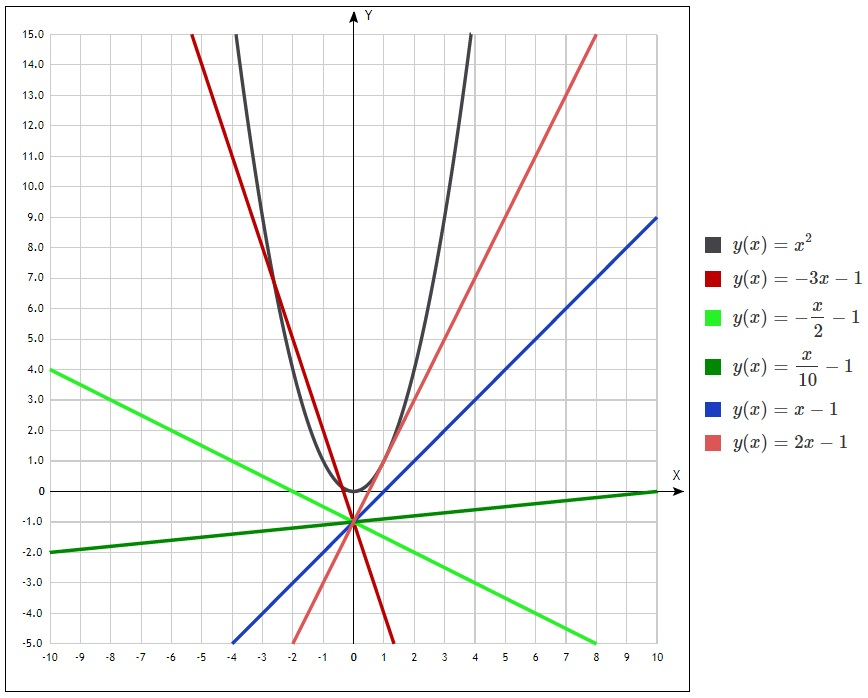
\includegraphics[width=\linewidth]{sol6}}
        \end{figure}
    \end{minipage}
\end{minipage}\vspace{1mm}\\
Таким образом, понимая что $|k| \geqslant 2$ нам не подходит, мы приходим к тому же ответу, что и в первом решении. Однако отмечу, что решая задачу графически, мы не предоставили никакого строгого доказательства о том, где происходит касание и почему. Данный способ решения надо \textbf{всегда} комбинировать с алгебраическим методом, так как сам по себе он доказательством не является~--- зато даёт понять, что происходит (в данном случае это вращение прямой вокруг точки $(0; -1)$)}
{Общих точек у прямой и параболы нет при $k \in (-2; 2)$.}{Как связано число точек пересечения графиков этих функций\\ с дискриминантом некоторого квадратного уравнения?}
\end{problem}

\begin{problem}{Уравнения с параметром.}{8.6.9}{9D}{(лёгкая)}
{Составить уравнение прямой, которая проходит через точку $A(0; 7)$ и касается окружности $(x - 15)^{2} + (y - 2)^{2} = 25$.}
{НаписанноеРешение}
{ВерныйОтвет}{Подсказка}
\end{problem}

\begin{problem}{Уравнения с параметром.}{8.6.9}{9D}{(лёгкая)}
{Составить уравнение окружности с центром в точке $M(3; 2)$, касающейся прямой $y = 2x + 6$.}
{НаписанноеРешение}
{ВерныйОтвет}{Подсказка}
\end{problem}

\begin{problem}{Уравнения с параметром.}{8.6.9}{9D red мб это слишком геома}{*}
{Точка $M$ лежит на прямой $3x - 4y + 34 = 0$, а точка $N$~--- на окружности $x^{2} + y^{2} - 8x + 2y - 8 = 0$. Найти наименьшее расстояние между точками $M$ и $N$.}
{НаписанноеРешение}
{ВерныйОтвет}{Подсказка}
\end{problem}

\begin{problem}{Уравнения с параметром.}{8.6.9}{9D red мб это слишком геома}{*}
{Найти наименьшее значение выражения $|a + b| + \sqrt{(a - 1)^{2} + (b - 3)^{2}}$.}
{НаписанноеРешение}
{ВерныйОтвет}{Подсказка}
\end{problem}

\begin{problem}{Уравнения с параметром.}{8.6.9}{9D}{*}
{При каких значениях $a$ все решения уравнения $\displaystyle \frac{2a - 3}{x + 2} = \frac{3x - 1}{((x - 2)^{2} + x - 14)}$\\ принадлежат отрезку $[-3; 4]$?}
{НаписанноеРешение}
{ВерныйОтвет}{Подсказка}
\end{problem}

\begin{problem}{Уравнения с параметром.}{8.6.9}{9D}{(лёгкая)}
{Найти все значения $a$, при которых система уравнений
$\;\left\{
\begin{aligned}
    (xy + x &+ y)(y + x^{2}) = 0\\
    y &= ax - 1
\end{aligned}\right.$ \\ имеет ровно два различных решения.}
{НаписанноеРешение}
{ВерныйОтвет}{Подсказка}
\end{problem}

\begin{problem}{Уравнения с параметром.}{8.6.9}{9D}{(лёгкая)}
{Построить график функции $\displaystyle y = \frac{2x + 1}{2x^{2} + x}$ и определить, при каких значениях\\ параметра $k$ прямая $y = kx$ имеет с графиком ровно одну общую точку.}
{НаписанноеРешение}
{ВерныйОтвет}{Подсказка}
\end{problem}

\begin{problem}{Уравнения с параметром.}{8.6.9}{9D}{(лёгкая)}
{Известно, что для всех действительных $x$ верно неравенство $(a + 5)x^{2} + (1 + 2a)x + (a - 7) \geqslant 0$. Чему может быть равно $a$?}
{НаписанноеРешение}
{ВерныйОтвет}{Подсказка}
\end{problem}

\begin{problem}{Уравнения с параметром.}{8.6.9}{9D}{(лёгкая)}
{Определить, при каких $a$ уравнение $\displaystyle x^{4} + \left(a + \frac{1}{3}\right)x^{2} + \frac{a}{3} = 0$ имеет 4 корня.}
{НаписанноеРешение}
{ВерныйОтвет}{Подсказка}
\end{problem}

\begin{problem}{Уравнения с параметром.}{8.6.9}{9D}{(лёгкая)}
{Определить, при каких $a$ уравнение $\displaystyle x^{4} - \left(1 - 5a\right)x^{2} - 5a = 0$ имеет 4 корня.}
{НаписанноеРешение}
{ВерныйОтвет}{Подсказка}
\end{problem}

\begin{problem}{Уравнения с параметром.}{8.6.9}{9D}{(лёгкая)}
{Определить, при каких $a$ уравнение $\displaystyle x^{4} + \left(2a - 5\right)x^{2} - 8a + 4 = 0$ имеет 4 корня.}
{НаписанноеРешение}
{ВерныйОтвет}{Подсказка}
\end{problem}

\begin{problem}{Уравнения с параметром.}{8.6.9}{9D}{(лёгкая)}
{Определить, при каких $a$ уравнение $\displaystyle x^{4} + \left(5a - 3\right)x^{2} - 15a = 0$ имеет 4 корня.}
{НаписанноеРешение}
{ВерныйОтвет}{Подсказка}
\end{problem}

\begin{problem}{Уравнения с параметром.}{8.6.9}{9D}{(лёгкая)}
{Определить, при каких $a$ уравнение $\displaystyle x^{4} - \left(3a + 4\right)x^{2} + 2a^{2} + 7a + 3 = 0$ имеет 4 корня.}
{НаписанноеРешение}
{ВерныйОтвет}{Подсказка}
\end{problem}

\begin{problem}{Уравнения с параметром.}{8.6.9}{9D}{(лёгкая)}
{Найти значения $a$, при которых неравенство $\displaystyle \left(a + 2\right)x^{2} + (a + 5)x + (a + 3) \leqslant 0$ будет выполнено для всех действительных $x$.}
{НаписанноеРешение}
{ВерныйОтвет}{Подсказка}
\end{problem}

\begin{problem}{Уравнения с параметром.}{8.6.9}{9D}{(лёгкая)}
{Найти значения $a$, при которых неравенство $\displaystyle \left(a + 5\right)x^{2} + (2a + 5)x + (a - 10) \leqslant 0$ будет выполнено для всех действительных $x$.}
{НаписанноеРешение}
{ВерныйОтвет}{Подсказка}
\end{problem}

\begin{problem}{Уравнения с параметром.}{8.6.9}{9D}{(лёгкая)}
{Найти значения $a$, при которых неравенство $\displaystyle \left(a - 3\right)x^{2} - (a - 2)x + (a + 6) \geqslant 0$ будет выполнено для всех действительных $x$.}
{НаписанноеРешение}
{ВерныйОтвет}{Подсказка}
\end{problem}

\begin{problem}{Уравнения с параметром.}{8.6.9}{9D}{(лёгкая)}
{При каком значении параметра $m$ неравенство $\displaystyle 3x^{2} + mx + 16 \geqslant 0$ выполняется для любого $x$?}
{НаписанноеРешение}
{ВерныйОтвет}{Подсказка}
\end{problem}

\begin{problem}{Уравнения с параметром.}{8.6.9}{9D}{(лёгкая)}
{Сколько корней имеет уравнение $x^{2} + 8x + 14 = |2x + 8| + a$ в зависимости от $a$?}
{НаписанноеРешение}
{ВерныйОтвет}{Подсказка}
\end{problem}

\begin{problem}{Уравнения с параметром.}{8.6.9}{9D}{(лёгкая)}
{Решить уравнение $(x^{2} + 1)^{2} - (2a + 3)(x^{2} + 1) + a^{2} + 3a = 0$.\\ Найти значения параметра $a$, при которых \\a) уравнение имеет $4$ корня; \hfill b) уравнение имеет $3$ корня;\\ c) уравнение имеет $2$ корня; \hfill d) уравнение имеет $1$ корень.

}
{НаписанноеРешение}
{ВерныйОтвет}{Подсказка}
\end{problem}

\begin{problem}{Уравнения с параметром.}{8.6.9}{9D red многопунктовая}{(лёгкая)}
{Найти значения параметра $k$, при которых уравнения имеют ровно один корень:
\\a) $9x^{2} - 2x + k = 6 - kx$ \\b) $3kx^{2} - 6x + k - 2 = 0$}
{а) Перенесем все в левую часть и сгруппируем подобные слагаемые:\\
$9x^2+(k-2)x+k-6=0$. Уравнение будет иметь единственное решение, если дискриминант $D=0$.\\
$D = (k-2)^2-(k-6)\cdot4\cdot9 = k^2-40k+220 = 0$. Решаем квадратное уравнение при $k$ получаем два корня: $k_1 = 20+6\sqrt{5}$ и $k_2 = 20-6\sqrt{5}$.\\
б) Аналогично, уравнение будет иметь единственное решение, если дискриминант $D = 0$, либо когда $k = 0$.\\
$D = 36 - 4\cdot(k-6)\cdot3k = k^2-2k-1 = (k-1)^2 \;\Rightarrow\; k = 1$, $k = = 0$. }
{а) $k = 20+6\sqrt{5}$ и $k = 20-6\sqrt{5}$. б) $k = 1$.}{Уравнение имеет единственное решение, если это или линейное уравнение, или квадратное уравнение, имеющее нулевой дискриминант.}
\end{problem}

\begin{problem}{Уравнения с параметром.}{8.6.9}{X}{*}
{Решить уравнение: $\;|a(x^{2} - 1)| = |2x - 3|$.}
{НаписанноеРешение}
{ВерныйОтвет}{Подсказка}
\end{problem}

\begin{problem}{Уравнения с параметром.}{8.6.9}{X}{(лёгкая)}
{При каких значениях $b$ уравнение $2x^{2} - bx + 8 = 0$ имеет два различных корня?}
{Квадратное уравнение имеет два различных корня при значении дискриминанта $D > 0$. В нашем случае получается:\\
$D = b^2-4 \cdot 8 \cdot 2 = b^2-64$. Значит $b^2-64 > 0 \;\Rightarrow\; b^2 > 64 \;\Rightarrow\; b \in (-\infty;-8)  \cup  (8;+\infty)$.}
{При значениях $b$ из интервала $(-\infty;-8)  \cup  (8;+\infty)$ уравнение будет иметь 2 различных корня.}{Квадратное уравнение имеет два различных корня лишь в том случае, когда дискриминант $> 0$.}
\end{problem}

\end{document}